\documentclass[fontsize=12pt, paper=a4, headinclude, twoside=false, parskip=half+, pagesize=auto, numbers=noenddot, open=right, toc=listof, toc=bibliography]{scrreprt}

%\usepackage[inner=4cm,outer=2cm]{geometry}
%\setlength{\oddsidemargin}{15,5pt}
%\setlength{\evensidemargin}{15,5pt}


%parskip:
  % full - Absätze haben großen Abstand
  % half - Absätze haben kleinen Abstand
  % off - Absätze haben Einzug (default)

% Bessere Unterstützung für PDF-Features
\usepackage[breaklinks=true]{hyperref}

%Schönere Schriftart laden
%\usepackage[latin1]{inputenc}
\usepackage[T1]{fontenc} % Ligaturen, richtige Umlaute im PDF
\usepackage[utf8]{inputenc}% UTF8-Kodierung für Umlaute usw
\usepackage[english]{babel} % Deutsche Silbentrennung verwenden
\usepackage{lmodern}
\renewcommand*\familydefault{\sfdefault}  %Zusatz für serifenlose Schrift.

%Zeilenabstand
\usepackage{setspace} % Zeilenabstand
\onehalfspacing % 1,5 Zeilen

% Schriften-Größen
\setkomafont{chapter}{\Huge\rmfamily} % Überschrift der Ebene
\setkomafont{section}{\Large\rmfamily}
\setkomafont{subsection}{\large\rmfamily}
\setkomafont{subsubsection}{\large\rmfamily}
\setkomafont{chapterentry}{\large\rmfamily} % Überschrift der Ebene in Inhaltsverzeichnis
\setkomafont{descriptionlabel}{\bfseries\rmfamily} % für description Umgebungen
\setkomafont{captionlabel}{\small\bfseries}
\setkomafont{caption}{\small}



% Einfachere Verwendung von korrekten Anführungszeichen
\usepackage[german=guillemets]{csquotes}
% oder german=quotes
% oder english=british oder english=american

%Mathematisches
\usepackage{amssymb}
\usepackage{amsmath}
\usepackage{amsthm}

%Quelltext einbinden
\usepackage{algorithm}
\usepackage{algorithmic}

%Abbildungen
\usepackage{graphicx}
\usepackage{caption}
\usepackage{subcaption}
\usepackage[verbose]{wrapfig}
\usepackage{float}
%\restylefloat{figure} %kannst du einen weiteren Positionierungsparameter [H] definieren. der setzt dir das bild an genau die stelle, wo du es haben willst. Ist allerdings auch nicht immer so praktisch.
% wenn du ein \pagebreak einfügst, gibt er dir vor der neuen seite noch alle gleitobjekte aus, die noch anstehen

%Zeichnen mit Tikz
\usepackage{tikz}
\usetikzlibrary{intersections,positioning,shapes.geometric,calc}

% Tabellen
\usepackage{multirow} % Tabellen-Zellen über mehrere Zeilen
\usepackage{multicol} % mehre Spalten auf eine Seite
\usepackage{tabularx} % Für Tabellen mit vorgegeben Größen
\usepackage{longtable} % Tabellen über mehrere Seiten
\usepackage{array}

%Bibliographie
\usepackage[square, comma, numbers, sort&compress, round]{natbib}
\usepackage{bibgerm} % Umlaute in BibTeX

%Umbenennung der vordefinierten definition- und example-Umgebung
\theoremstyle{definition}
\newtheorem{lecture}{Lecture}
\newtheorem{definition}{Definition}
\newtheorem{example}{Example}
\newtheorem{lemma}{Lemma}

% \newtheorem{theorem}{Satz}
% \newtheorem{constructing instructions}{Konstruktionsvorschrift}
% \newtheorem{properties}{Eigenschaften}
%\newtheorem{proposition}{Proposition}
%\newtheorem{korollar}{Corollary}
%\newtheorem{remark}{Remark}
%\newtheorem{consequences}{Consequences}
%\newtheorem{observation}{Observation}
%\newtheorem{conjecture}{Conjecture}
%\newtheorem{recall}{Recall}

\renewcommand{\labelenumi}{\roman{enumi})}

\renewcommand{\labelitemii}{$\bullet$}

\newcommand{\todo}[1]{
      {\colorbox{red}{ TODO: #1 }}
}
\newcommand{\todotext}[1]{
      {\color{red} TODO: #1} \normalfont
}

%bzgl `tocbasic` Warnung
\usepackage{scrhack}
 % Importiere die Einstellungen aus der Präambel
% hier beginnt der eigentliche Inhalt

\author{Lydia Buntrock}
\title{master thesis}
\date{Januar 2018}

\hfuzz=\maxdimen \tolerance=10000 \hbadness=10000
% \usepackage[showframe=true]{geometry}


\begin{document}
  % Titelseite
  \begin{titlepage}
    \pagestyle{empty}
  	\begin{center}
      {\Large Freie Universität Berlin} \\
    	\begin{Huge}
      	Fachbereich Mathematik und Informatik \\
      	\vspace{3mm}
    	\end{Huge}
    	\vspace{2cm}
    	\begin{Large}
        \textbf{An analysis of maximum parsimony algorithms to predict parasitism in Eukaryota} \\
        \vspace{3mm}
        using a large multifurcated phylogenetic synthesis tree \\
    	\end{Large}
      \vspace{3cm}
      \textbf{Eingereicht am:} \\
      3.4.2018 \\
    	\vspace{2cm}
    	Lydia Buntrock \\
      E-Mail: info@irallia.de \\
     	\vspace{3cm}
      \textbf{Betreuer:} \\
      Dr. Bernhard Y. Renard \\
      \& \\
      Prof. Dr. rer. nat. Emanuel Heitlinger \\      
  	\end{center}
  	\clearpage
  \end{titlepage}

%---------------------------------------------------------------------------------------------------
%---------------------------------------------------------------------------------------------------
%---------------------------------------------------------------------------------------------------
%--------------------------------------------------------------------------------------------------- 
\chapter*{Abstract}

% Parasitism in Eukaryota - Reconstruction of ancestral and unavailable extant states

% Lydia Buntrock^1; Jorrit Poelen^?; Berhard Renard^2; Emanuel Heitlinger^1,3;

% 1 - Institute for Biology, Molecular Parasitology, Humboldt University, Berlin, Germany
% 2 - Bioinformatics Unit (MF1), Department for Methods Development and Research Infrastructure, Robert Koch Institute, Berlin, Germany
% 3 - Research Group Ecology and Evolution of Molecular Parasite Host Interactions, Leibniz Institute for Zoo and Wildlife Research, Berlin, Germany

% ## Wenn du willst kannst du auch das IZW (3) an deinen Namen heften!
% ## Yorrit bitte das Abstract schicken und fragen ob er Co-Author sein will. 

  Parasitism can be defined as an interaction between species in which one of the interaction 
    partners, the parasite, lives in or on the other, the host. The parasite draws food from its 
    host and harms it in the process. According to some estimates, above 50\% of all eukaryotes are 
    parasites. Nevertheless, it is difficult to obtain information whether a particular taxon is a 
    parasite computationally making it difficult to query large sets of taxa. \\

  Here we test in how far it is possible to use the open tree of life (OTL), a synthesis of 
    phylogenetic trees on a backbone taxonomy (resulting in unresolved nodes), to expand available 
    information via phylogenetic trait prediction. We use the Global Biotic Interactions (GloBI) 
    database to categorise 25,992 and 34,879 species as parasites and free-living, respectively and 
    predict states for over ~2.7 million (97.6\%) leaf nodes without state information. \\

  We estimate the accuracy of our maximum parsimony based predictions using cross-evaluation and 
    simulation at roughly 80\% overall, but strongly varying between clades. We describe this 
    variation across taxa as associated with available state and topology information. We compare 
    our results with several smaller scale studies, which used manual expert curation and conclude 
    that computationally inferred state changes largely agree in number and placement with those. In 
    clades in which available state information is biased (mostly towards parasites, e.g. in 
    Nematodes) phylogenetic prediction is bound to provide results contradicting conventional 
    wisdom. \\

  This represents, to our knowledge, the first comprehensive computational reconstruction of the 
    emergence of parasitism in eukaryotes. We argue that such an approach is necessary to allow 
    further incorporation of parasitism as an important trait in species interaction databases and 
    in individual studies on eukaryotes e.g. in the microbiome. \\

  ------------ \\

  This study focuses on the ancestral state reconstruction of parasitism in the tree of life of
    Eukaryota. We predict unknown states of species and estimate origins and losses of parasitism. \\
  The challenge here is the size of the tree and the little information about it. \\
  Such a large phylogenetic tree does not completely exist and therefore we work with a synthesis 
    tree of OTL \cite{Hinchliff2015} which is highly multifurcated. \\
  For the 2,535,437 leaf nodes we could not gather much data. From the GloBI database 
    \cite{Poelen2014} which we used, we could only collect 25,992 parasitic and 34,879 
    free-living species. It follows that we have only $\approx 2.4~\%$ state information. \\
  So far, especially small scale studies have been carried out or highly manual. In this scale, it 
    requires different data sources to be interconnected. \\
  We performed an analysis of existing algorithms and selected a Sankoff maximum parsimony algorithm 
    using the R package \textit{Castor} \cite{Louca2017}. \\
  Nevertheless, the results are convincing and even though purely computational approach which did 
    not include human experts input, results coincide with prior knowledge. Also regarding the number 
    of events, our estimates coincide with previous results by human experts, e.g. the study by 
    Weinstein and Kuris \cite{Weinstein2016}. \\

  ------------ \\

  \anmerkungstext{Klassisch packt man keine Referenzen in Abstracts (bzw. wenn das meist als 
    Kurzreferenz also (Author et al., 2017). (Bernhard)} \\
  We have compared the results of some subtrees with known knowledge (Chordata, Nematoda, 
    Platyhelminthes and Apicomplexa) and, except for the Nematoda, the results looked very good. In 
    the case of Nematoda, the data situation is strongly shifted to the few parasites. \\
  We could partly compare our number of origins with the results of Sara B. Weinstein and Armand M. 
  Kuris from their article \textit{Independent origins of parasitism in Animalia}  
    and have come to a similar magnitude. They identified 223 parasitic origins in Metazoa and we 
    were able to estimate about 300 origins. \\

\tableofcontents
\clearpage

%---------------------------------------------------------------------------------------------------
%---------------------------------------------------------------------------------------------------
%---------------------------------------------------------------------------------------------------
%--------------------------------------------------------------------------------------------------- 
\chapter{Introduction}
  This paper is about the analysis of ancestral state reconstruction algorithms for non-binary trees, 
    applied to the currently largest phylogenetic synthesis tree of Open Tree Of Life (OTL)
    \cite{Hinchliff2015}, with the application of prediciton of parasitism. \\
  % \todo{Or:} The aim of this paper is the application of maximum parsiomony algorithms to non-binary 
  %   trees and very large datasets. In particular, the example 'Origins of Parasitism' throughout the 
  %   Eukaryota Tree of Life. \\

  We will test the existing maximum parsimony algorithms Fitch \cite{Fitch1971} and Sankoff 
    \cite{Sankoff1975} for this task and estimate their predictive power. The present tree structure 
    of OTL is not binary. A tree is binary (or bifurcated), when each node has at most two children 
    otherwise it is multifurcated \cite{Felsenstein2003}. \\
  % \anmerkungstext{auch hier kannst du multiifurcated direkt erklären: that is it each not has 
    % multiple (n >= 3) children (Thilo)}
  Maximum parsimony methods are developed for phylogenies, which are usually depicted as binary trees.
    Parsimonious in phylogeny refers to favoring the tree that needs the least evolutionary change 
    to explain the observed data. In our case, it is about the change of states 'is free-living' or 
    'is parasitic'. \\
    % Parsimonious in this context means to minimize the number of transitions between species states 
    % (free-living or parasitic). 
  The Sankoff method is implemented by Louca et al. for the non-binary case and is available as an R 
    package called \textit{Castor} \cite{Louca2017}. In addition, we have implemented the Fitch 
    method and adapted it for multifurcated trees. \\% to make it usable and comparable for our current problem.
  This achieves that we can predict ancestral states and unknown states of living species for large 
    non-binary relatives trees. \\

  For about 50 years, people have been working on ancestral state reconstruction. The first paper 
    is by Camin and Sokal, who in 1965 were working on algorithms for discrete-state data 
    \cite{Camin1965}. Different methods have been developed and the question is which method is the 
    most suitable for the problem at hand: The ancestral state reconstruction for a huge 
    multifurcated tree with \colorbox{red}{binary/two discrete} states. \\
  \anmerkungstext{hier mehr dazu? Likelihood vs parsiomony... das befindet sich momentan im Methoden 
    Teil: Ancestral state reconstruction methods} \\
  % Royer-Carenzi et al. distinguishes two major classes of ancestral state reconstruction methods: \\
  %   The first is to explain the current state with the least number of state changes between an 
  %     ancestor and his child, this is called parsimonious. \\
  %   The other class she presents involves modeling the character evolution as a stochastic process and 
  %     using the likelihoods to compute the possible ancestral character states. This is generally done 
  %     with a continuous time Markov model \cite{RoyerCarenzi2013}. \\
  
  % The first methods were only brute force \todo{Quelle, siehe Fitch: Camin and Sokal 1965}. 
  %   Next came a set of parsimony algorithms such as: Fitch-parsimony \cite{Fitch1971}, 
  %   Wagner-parsimony \cite{Swofford1987} ... \todo{weitere?}. \\
  %   With more and more data, there is now the possibility to use more information to calculate the 
  %   probabilities of the ancestral states. In addition to the states of the leafs, algorithms could 
  %   also use branch lengths. The likelihood based algorithms came more in interest. \\
  
  % We have decided to consider only parsimony algorithms since we have no information on branch 
  % lengths and no other additional information like different transition probabilities of our states.

  For this purpose, various studied methods and their advantages and disadvantages will be compared. \\
  These algorithms were developed especially for the binary problem, since one has considered much 
    smaller subtrees, of which one knows all the splits. \\
  By developing a whole of an entire tree of life, the problem arises that it is by no means binary. \\

  For these large phylogenetic synthesis trees, however, ancestral state reconstruction has so far 
    only been done for Bacteria and Archaea for binary traits by Goberna and Verdú \cite{Goberna2015}.
    However, this differs from eukaryotes in the sense that complex traits such as parasitism depend
    on more than one gene. \\

  To accomplish this task, a large phylogenetic tree and information about the current species states 
    is needed. \\
  The biggest 'phylogenetic tree' is a synthesis of phylogenetic trees filled with a taxonomic trees 
    given by Open Tree of Life (OTL) \cite{Hinchliff2015}. %This tree is not binary and therefore the 
    % developed algorithms are not directly applicable. Therefore, an algorithm must be found that can 
    % work with non-binary trees. \\
  For the information about the current states of the species we use the interaction database Global 
    Biotic Interactions (GloBI) \cite{Poelen2014}. The data in GloBI are stored as interactions e.g. 
    species A parasitize species B. From this we conclude that species A is parasitic and species B 
    free-living. \\

  At this point a few words to the term parasitic. There are different definitions. Since we use 
    GloBI to classify species, we use their definition of parasitism. Again, in GloBi, Ontobee 
    definitions are used \cite{Xiang2011}.
  The interaction \textit{has parasite} is defined as: "An interaction relationship between two 
    organisms living together in more or less intimate association in a relationship in which 
    association is disadvantageous or destructive to one of the organisms." \cite{...}. This 
    definition includes: ecto- and endoparasites, parasitoids, kleptoparasites and pathogenes.
  \todotext{Mungall, C., (2017). Definition for the interaction-term: "parasitised by; has parasite" 
  ob ontobee.org. Last checked: 24.07.2017 at 
  \hyperlink{ontobee.org/ontology/RO?iri=http://purl.obolibrary.org/obo/RO_0002445}
  {ontobee.org/ontology/...}} \\

  The objectives of this work are the following points: (1) Find a suitable ancestral state 
    reconstruction method. (2) Perform reconstructing on the Eucaryotic synthesis tree of OTL. \\
  The goal of Point 1 is to evaluate the possible methods based on a simulation of our data 
    situation. \\
  The one by Louca et al. implemented Sankoff algorithm is the best in our comparisons. Therefore, 
    point 2 consists of reconstructing the ancestral states and predicting the unknown leaf states. 
    And then perform an evaluation of the results.

%---------------------------------------------------------------------------------------------------
%---------------------------------------------------------------------------------------------------
%---------------------------------------------------------------------------------------------------
%--------------------------------------------------------------------------------------------------- 
\chapter{Methods}
  As initiated, in this paper, a maximum parsimony algorithm is applied to the whole tree of life to 
    obtain an ancestral state reconstruction of free-living versus parasite states. \\
  So far, these reconstructions have been made mainly on binary trees with better data availability. 
    Therefore, a simulation is first performed to evaluate existing algorithms and decide how they 
    may be adapted to our given problem. This is to perform the ancestral state reconstruction for a 
    multifurcated (non-binary) tree using binary states. \\
  Accordingly, in addition to the necessary data sets (GloBI, OTL), the chosen algorithm and the 
    evaluation of its results, this chapter also deals with the previously performed simulation and 
    the evaluation of the various algorithms and their parameters. \\
  Figure \ref{fig:workflow} briefly outlines these relationships.
  \begin{figure}[h!]
    \centering
    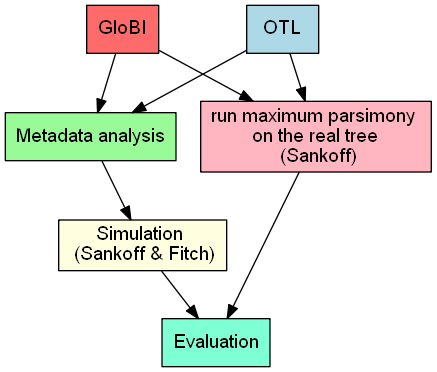
\includegraphics[width=0.5\textwidth]{Figures/Workflow-overview.png}
    \caption{Workflow \\
      The resulting procedure is as follows: \\
      (1) Retrieve phylogenentic tree data as input for the tree (OTL) and the state information (GloBI).
      (2) Get metadata of these for a realisitc the simulation of the maximum parsimony algorithms (Fitch \& Sankoff).
      (3) Build and run the simulation.
      (4) Evaluation of parameters for the simulation and the ancestral state reconstruction of the real tree.
      (5) Evaluate the accuracy of developed algorithms and choose the best.
      (6) Run the resulted algorithm on the original data.
      (7) Evalute and interprete results. %$\rightarrow$ Origins etc...
    }
    \label{fig:workflow}
  \end{figure}

  \todo{In den einzelnen Abschnitten Teile von dem großen Workflow verwenden?: \ref{fig:BigWorkflow}}

  %---------------------------------------------------------------------------------------------------
  %---------------------------------------------------------------------------------------------------
  %---------------------------------------------------------------------------------------------------
  \section{Description of data sets}
    For \colorbox{red}{our} research two types of data are required: a tree and information about the 
      states. \\
    For the tree \colorbox{red}{we} decided to use Open Tree of Life (OTL) \cite{Hinchliff2015}. \\
    For the state information, \colorbox{red}{we} decided to use the Global biotic interaction 
      database (GloBI) \cite{Poelen2014}.

    %---------------------------------------------------------------------------------------------------
    %---------------------------------------------------------------------------------------------------
    \subsection{OTL}
      For \colorbox{red}{our} project a large database for phylogenetic trees and also for a taxonomic 
        tree is needed. Since an ancestral state reconstruction algorithm is applied to the phylogenetic 
        tree, and for the assessment and other properties the taxonomy provides much more information. \\
      OTL gives a synthesis of phylogenetic trees (currently 819 trees) and a taxonomic tree. OTL also 
        includes the large phylogenetic database TreeBASE \cite{Hinchliff2015}. \\
      \todo{Das steht auf der Website nicht in dem Paper...} \\
      For phylogenetic data, there are at least five big data collections, namely:
      \begin{itemize}
        \item ITIS (Integrated Taxonomic Information System) \cite{ITIS}
        \item NCBI (National Center for Biotechnology Information) \cite{NCBI1988}
        \item WORMS (World Register of Marine Species) \cite{WoRMS2018}
        \item GBIF (Global Biodiversity Information Facility) \cite{GBIF}
        \item OTT (OpenTreeOfLife-Taxonomy) \cite{Hinchliff2015}
      \end{itemize}
      \todo{In die discussion?:} \\
      ITIS is only a small set of 100~\% confirmed and named species. GBIF is not composed with the help 
        of phylogeny, the same is valid for the NCBI taxonomy. The WORMS taxonomy is a way too small 
        dataset of mostly marine species. \\
      Here the taxonomy from OTL is used because it is including most of the known taxonomies and is 
        synthesised by preffering taxonomies that match with available phylogenetic data. Furthermore 
        the team from OTL preferre a maximum number of species \cite{Hinchliff2015}. This is resulting 
        in somekind of hybrid between taxonomy and phylogeny. \anmerkungstext{Wie genau ist das ein 
        Hybrid? Genauer beschreiben, was Du damit meinst... (Thilo)} \\

      A closer look is being made to some of the features of the synthesis tree. On the one hand the 
        distribution of the taxa and on the other the distribution of the nodes on the taxa. Since this 
        is not directly relevant to \colorbox{red}{our} study, there is a section in the appendix 
        \ref{sec:otl analysis}.

    %---------------------------------------------------------------------------------------------------
    %---------------------------------------------------------------------------------------------------
    \subsection{GloBI}
      \todotext{Marius:} "There aren't many big active interaction databases out there, most of them are 
        offline or outdated. For example: IWDB (Interaction Web Database) \cite{IWDB2003}, Webs on the 
        Web \cite{WOW2004}, Animal Diversity Web \cite{Myers2003} and ecoweb \cite{Cohen2010}. GloBI is 
        including most of the known ones and is still growing actively \cite{Poelen2014}. So the 
        question which interaction database could be used was answered rather quickly." \\

      This database consists of entries of the form: species A (source) interacts with B (target). \\
      A number of interactions have been identified\footnote{\hyperlink{
        https://github.com/jhpoelen/eol-globi-data/blob/master/eol-globi-lib/src/main/java/org/eol/globi/domain/InteractType.java
        }{https://github.com/jhpoelen/eol-globi-data/.../InteractType.java}}
        ,including those that the species source or target has become a parasite or a free-living 
        species from the biological perspective. These are the following:
      \begin{itemize}
        \item free-living source: preysOn, eats, flowersVisitedBy, hasPathogen, pollinatedBy, 
          hasParasite, hostOf
        \item free-living target: preyedUponBy, parasiteOf, visitsFlowersOf, pathogenOf, hasHost
        \item parasite source: parasiteOf, pathogenOf
        \item parasite target: hasParasite, hasPathogen
      \end{itemize}
      Of these interactions, e.g. species A parasitize species B, the state of the species is 
        determined, here is species A parasitic and species B free-living. The case a parasite 
        conquers (parasitizes) another parasite yields conflicting states for the second species. 
        This is solved by preferring parasitic. \\
      Two lists are formed: parasites and free-livings, and the source or targets of an interaction
        are added to these.

  %---------------------------------------------------------------------------------------------------
  %---------------------------------------------------------------------------------------------------
  %---------------------------------------------------------------------------------------------------
  \section{Metadata analysis}
    In order to generate a realistic simulation, influencing parameters are investigated. \\
    There are two major types of parameters:
    \begin{enumerate}
      \item Biological parameters (A result of the evolutionary process.):
        \begin{itemize}
          \item transition probabilities
        \end{itemize}
      \item Distribution of the loss of information:
        \begin{itemize}
          \item Loss of topology ($\rightarrow$ mutlifurcations)
          \item Unknown information about states of some leaf nodes
        \end{itemize}
    \end{enumerate}
    The influence of these parameters are tested on our result using our simulation (Section 
      \ref{sec:simulation}).
   
    %---------------------------------------------------------------------------------------------------
    %---------------------------------------------------------------------------------------------------
    \subsection{Transition probabilities}
      This subsection deals with the transition probabilities from free-living (hereinafter / as a 
        formula FL) to parasitic (hereinafter P) and vice versa: $\mathcal{P}(FL \rightarrow P)$, 
        $\mathcal{P}(P \rightarrow FL)$. \\
      Different parasite types have different transition probabilities. It is very difficult to make a 
        statement about these probabilities.
      In general, \colorbox{red}{we} assume that there are 40~\% parasites and 60~\% free-livings which 
        is based on the estimates by Windsor \cite{Windsor1998} and 
        $\mathcal{P}(FL \rightarrow P) > \mathcal{P}(P \rightarrow FL)$, because a reverse mutation is 
        usually less likely. \todo{This is discussed in section x of the discussion.} \\

      For the maximum parsimony analysis of the real data, all transition probabilities are equated.
        However, the used castor package \cite{Louca2017} offers the possibility to enter different 
        transition probabilities.
      \begin{wrapfigure}{r}{0.5\textwidth}
        \begin{center}
          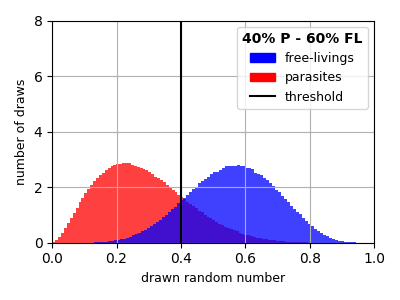
\includegraphics[trim = 0mm 0mm 0mm 13mm, clip, width=0.48\textwidth]{Figures/40-60.png}
        \end{center}
        \caption{60~\% Free-living - 40~\% Parasites \\ red: parasites, blue: free-living, \\ the threshold is at 0.4}
        \label{fig:Beta distribution}
      \end{wrapfigure}

      In the simulation two beta distributions have been chosen and a threshold that indicates the change 
        between states. \\
      Different thresholds with different beta distributions are simulated, with different distributions 
        of parasites and free-livings:
        \begin{itemize}
          \item 50~\% P to 50~\% FL,
          \item 40~\% P to 60~\% FL,
          \item 30~\% P to 70~\% FL and 
          \item 20~\% P to 80~\% FL
        \end{itemize}
        (\todo{see results simulation, ref...}). Figure \ref{fig:Beta distribution} 
        shows one example of these. \\
      \todo{Plot neu erstellen: Achsenbeschriftung, threshold}

    %---------------------------------------------------------------------------------------------------
    %---------------------------------------------------------------------------------------------------
    \subsection{Missing information}

      A binary tree with $n$ leaf nodes has $n-1$ internal nodes. The present Eukaryota tree of OTL has 
        2,293,463 leaf nodes and only 41,974 internal nodes, that is:
      $$100-\frac{100}{(2293463-1) \times 41974} \approx 98.16 \%$$
        missing internal nodes. This means that there is a lack of information about the underlying 
        phylogeny. Instead of a binary tree this tree is highly multifurcated. \\

      % \anmerkungstext{Nested models were compared using likelihood ratio tests, models using different 
      %   predictors were compared according to their deviance and AIC. (Emanuel)} \\

      For the present Eukaryota tree with 2,293,463 leaf nodes, 34,869 free-livings and 25,962 parasites 
        are found, which are
        $$100-\frac{100}{2293463 \times (34860+25962)} \approx 97.34 \%$$
        unknown states of leaf nodes. \\

      In the simulation, the influence of the multifurcation and missing data in leaf nodes on the 
        predictive accuracy of the ancestral state reconstruction algorithms is tested. \\
      For the real data, generalized linear models are compared with poisson respectively binomial 
        regression according to their residuals and BICs. \\
      \anmerkungstext{Erklären, warum und wozu das gemacht wird. Warum BIC und nicht AIC? Erklären,
        was beide bedeuten, wäre sinnvoll. (Thilo)} \\

      For each node, depth, min, max and mean height were noted. Where the depth of a node is the 
        distance (number of edges) to the root node and the height of a knot is described as the 
        largest distance to a leaf node. In this work, a distinction is made between minimum, maximum 
        and average distance ($\rightarrow$ min, max and mean height). \\
      The influence in the modeling of these parameters was tested, additive as well as multiplicative.

  %---------------------------------------------------------------------------------------------------
  %---------------------------------------------------------------------------------------------------
  %---------------------------------------------------------------------------------------------------
  \section{Simulation}\label{sec:simulation}
    There are various possibilities of ancestral state reconstruction. The simulation compares
      different algorithms with each other. \\
    First different implementations of the Fitch maximum parsimony are compared and then the best of 
      them is compared with the implementation of the sankoff algorithm of the castor package 
      \cite{Louca2017}. \\

    \begin{figure}[h!]
      \centering
      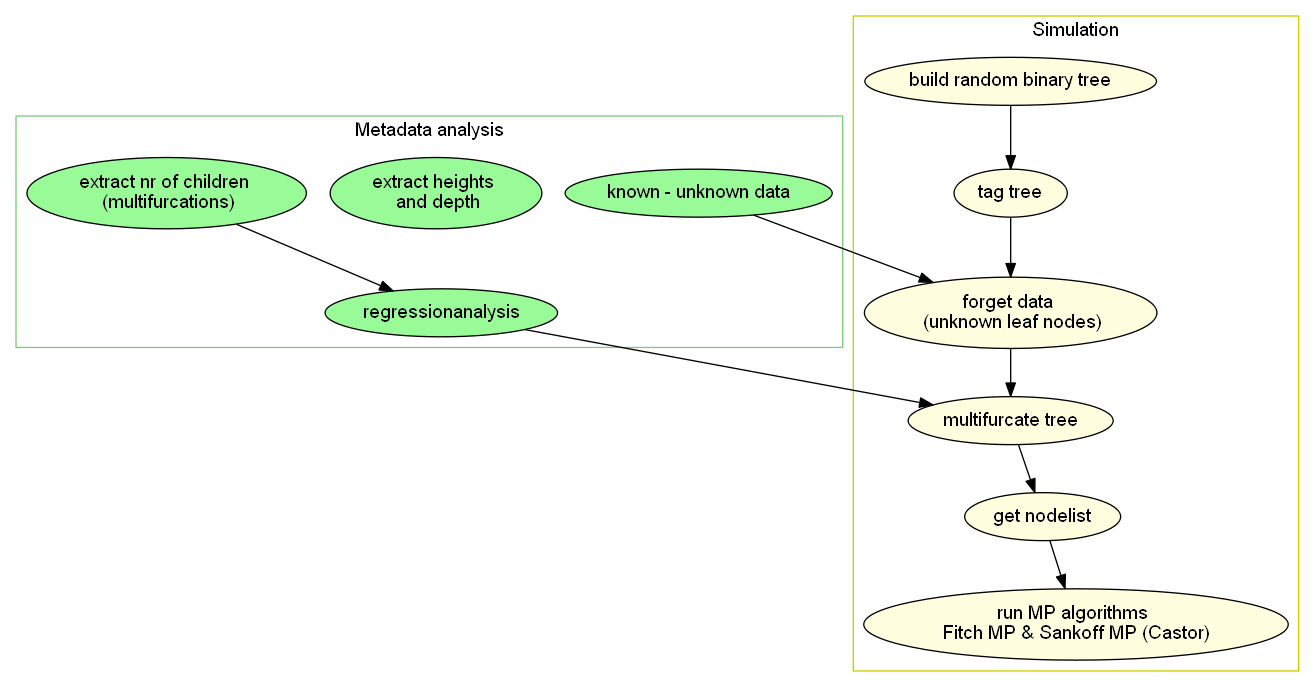
\includegraphics[width=1\textwidth]{Figures/Workflow-Simulation.png}
      \caption{Course of the simulation with influence of the metadata analysis from the real data.}
      \label{fig:Simulation Workflow}
    \end{figure}

    \todotext{Figure \ref{fig:Simulation Workflow} shows the course of the simulation. The individual 
      steps are explained in the following subsections: ...}

    \todo{Evaluation - compare trees (distances)}

    %---------------------------------------------------------------------------------------------------
    %---------------------------------------------------------------------------------------------------
    \subsection{random binary tree}
      A tree is needed to do a simulation of ancestral state reconstruction. It had to be decided whether 
        to take the real tree or simulate a tree. In this simulation, trees are created randomly, as 
        one can replicate a complete binary phylogentic tree. Thus, there is also the possibility to 
        simulate the multifurcation. \\
      
      To get a random binary tree, the Phylo package from biopython is used \cite{Cock2009}. They offer 
        a randomized function which returns a BaseTree\footnote{
          \hyperlink{https://github.com/biopython/biopython/blob/master/Bio/Phylo/BaseTree.py}
          {https://github.com/biopython/biopython/blob/master/Bio/Phylo/BaseTree.py}
        }. \\
      \todo{ref in die discussion über die randomized function? Diskutieren wir das?}

    %---------------------------------------------------------------------------------------------------
    %---------------------------------------------------------------------------------------------------
    \subsection{simulating states and transitions between them}
      The next step is to simulate the states of the nodes using the transitions. Again, fully known 
        states are simulated and then everything is 'forgotten' but a few in the leaf nodes so that 
        \colorbox{red}{you} can later compare the reconstruction with the origin. \\
      The root node is defined as ancestor of all subsequent species and in this case, determined to be
        free-living. Therefore, a beta distribution for free-living is used at the beginning. Now 
        traverse from the root to the leaf nodes, always pulling out of the current distribution until 
        \colorbox{red}{you} get above the threshold and the new node changes state. \anmerkungstext{Für 
        den Tree/Graph Traversal würde sich eine erklärende Abbildung anbieten. Nur Text macht es sehr 
        schwer verständlich an der Stelle. (Thilo)} \\
      To ensure that the parameter of the binomial distribution is restricted to the [0,1] interval, it 
        is modeled with a beta distribution as in Figure \ref{fig:Beta distribution}. \\

      After traversing through the tree, each state is saved in a nodelist associated with the node ID 
        which is the OTT from OTL. \\

% simulate loss of information
      Here begins the simulation of the lost information. This is on the one hand the states and on the 
        other the topology of the tree. Some splits of nodes are unknown with which the tree is 
        multifurcated (explained in the following section \todo{pageref}). \\

      In the real tree, there is usually only information about species living today $\rightarrow$ leaf 
        nodes. And beyond only a small percentage of these. All information about the states of the 
        internal node and one leaf node is 'forgotten' and stored in another column to the node. \\
      Different percentages of forgetting the information are simulated, as \colorbox{red}{you} can read 
      in the \todo{section ... from the results}.

    %---------------------------------------------------------------------------------------------------
    %---------------------------------------------------------------------------------------------------
    \subsection{simulating loss of information of the tree topology}
      As previously explained, some divisions in the tree are not known, so the real tree is not binary.
      This multifurcation was simulated by an equally distributed percentage of forgotten internal nodes.

    %---------------------------------------------------------------------------------------------------
    %---------------------------------------------------------------------------------------------------
    %---------------------------------------------------------------------------------------------------
    \section{Ancestral state reconstruction methods}
      As presented in the introduction, there are some methods for ancestral state reconstruction. For 
        this purpose, various studied methods and their advantages and disadvantages are compared below. \\
    
      Royer-Carenzi et al. distinguishes two major classes of ancestral state reconstruction methods: \\
      The first is to explain the current state with the least number of state changes between an 
        ancestor and his child, this is called parsimonious. \\
      The other class she presents involves modeling the character evolution as a stochastic process and 
        using the likelihoods to compute the possible ancestral character states. This is generally done 
        with a continuous time Markov model \cite{RoyerCarenzi2013}. \\
      \todo{Pasqualin et al. unterscheiden noch eine weitere Methode: stochastic mapping...} \\

      One of the major disadvantages of parsimony methods is that, unlike likelihood approaches, they 
        can not take divergece times (branch length) into account. Since there are no development times 
        of species in our case, \colorbox{red}{you} can ignore this. \\
      Another problem pointed out by Royer-Carenzi is that parsimony approaches are either based on 
        predefined parameters (generalized parsimony) or on strong and often controversial assumptions, 
        like irreversibility of transitions for dollo parsimony. Again, this problem is irrelevant to 
        the problem at hand, because \colorbox{red}{you} can only work with generalized models in the 
        analysis of the entire Eukaryota tree. \\

      Parsimony-based methods are used in this work, since they are fully sufficient for the presented 
        use case here. Following the principle of the simpler model first. \\
      Felsenstein \cite{Felsenstein2003} discusses in his book two algorithms that generalize all 
        previous methods (from Camin and Sokal \cite{Camin1965}, \todo{Kluge and Farris} and Farris 
        \cite{Farris1970}): Fitch parsiomony \cite{Fitch1971} and Sankoff parsimony \cite{Sankoff1975}. \\
      \anmerkungstext{Unter Farris war auch noch der Begriff Wagner trees in gebrauch, als 
        Verallgemeinerung der parsimonious trees von Camin und Sokal. (Lydia)} \\
      \todo{Wagner-parsimony \cite{Swofford1987}} \\
      
      Thus, the methods used in this work are those of Fitch and Sankoff. For Fitch, the algorithm has 
        been extended from binary to multifurcated trees. For the Sankoff algorithm, Louca and Doebeli 
        have presented an implementation for non-binary trees published in an R package named 
        \textit{castor} \cite{Louca2017}.

      %---------------------------------------------------------------------------------------------------
      %---------------------------------------------------------------------------------------------------
      \subsection{Fitch maximum parsimony}
        Fitch maximum parsimony is an algorithm for rooted, binary trees and describes an ancestral state 
          reconstruction for discrete states \cite{Fitch1971} by minimizing transitions between states. \\
        Note, the original Fitch algorithm has the sole purpose of minimizing the number of transitions 
          and not reconstructing the ancestral nodes. Felsenstein \cite{Felsenstein2003} describes a 
          simple extension for the reconstruction. Cunningham et al. \cite{Cunningham1998} have refined 
          these. \todotext{Wir haben mit ein paar kleinen änderungen optimiert... und schließlich auf 
          multifurcated angepasst...} \todotext{eigentlich ist Cunningham 'nur' eine kritische 
          Neubewertung. Sie beziehen ihren Algortihmus auf Swofford und Maddison...} \\
        To understand the differences to the multifurcated case, the algorithm for the binary case is 
          briefly explained and referred to the extension. \\

        Input: A rooted, binary tree, with state informations in the leaf nodes. Each node is depicted as 
          a set of states. There are only two states in this paper, free-living (FL) and parasitic (P). 
          Internal nodes have three sets, which are empty at the beginning, excluding the root node, it 
          has only one. Leaf nodes have their state as a set (eg \{FL\} or \{P\}, unknown leaf nodes the 
          union of all possible states (\{FL, P\}). \\
        The algorithm traverses three times trough the tree and fills these sets. \\
        In each step, two sets are considered and their intersect formed. There are two cases:
        \begin{enumerate}
          \item The intersection is not empty and corresponds to the new set.
          \item The intersection is empty. $\rightarrow$ Build the union of these sets as new set.
        \end{enumerate}

        First traverse from the leaf nodes to the root / move down the tree / postorder tree traversal.
          \begin{wrapfigure}{r}{0.5\textwidth}
            \centering
            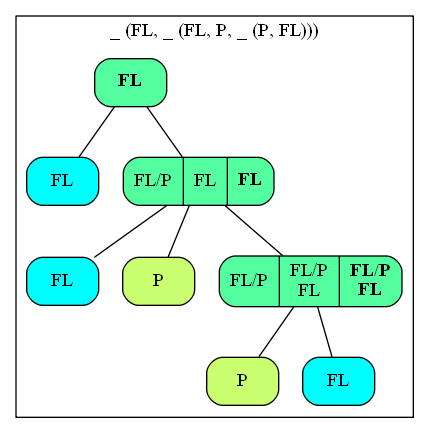
\includegraphics[width=0.4\textwidth]{Figures/Fitch1.png}
            \caption{Fitch algorithm for binary trees. \\
              The unknown leaf node is discribed with both states. Computed internal nodes (exclusive the 
              root node) consists of three sets, where the last set is the final one (bold). \\
              From the second internal node (seen from the root node) there are several possibilities to 
              create the second and third set.}
            \label{fig: binary Fitch}
          \end{wrapfigure} 
          Each internal node is formed from its child nodes, where at the beginning the only information
          lies. \\
        Second traverse from the root node to the leafs. Each internal node is formed from its father node 
          and its sibling node. \\
        Last traversion (direction does not matter): Build the final state for every node. It is formed 
          from the sets of previous traversals. \\
        (The original Fitch algorithm was designed to minimize transitions without predicting actual states 
          of internal nodes, so it was just the first traversal.) \\
        The extension to the non-binary case is quite obvious, but holds some opportunities. In this case, 
          more than two children may be present for the first traversal, but the incision or union may 
          also be formed over more than two sets. Also in the second traversing, there may be several 
          sibling nodes. However, there are several possibilities here that were all tested and compared 
          in the simulation. Some of these options are already available in the binary case:
        \begin{itemize}
          \item The father node has (except for the root node) two state sets, because he came through 
            the up-traversing previously. Are both sets used or only the first traversing?
          \item Since there are several siblings, do \colorbox{red}{you} first of all make the cut or union, 
            or directly in the whole with the father node?
        \end{itemize}
        The first point already has an effect on the binary case. Figure \ref{fig: binary Fitch} shows 
          both possibilities of the three sets. \\
        Cunningham uses only the first state set of the father node \cite{Cunningham1998}. \\
        From these two points four different versions of Fitch were formed:
        \begin{enumerate}
          \item Fitch 1: First state set of father node; intersection/union of siblings first.
          \item Fitch 2: First state set of father node; intersection/union of siblings together with father node.
          \item Fitch 3: Both state sets of father node; intersection/union of siblings first.
          \item Fitch 4: Both state sets of father node; intersection/union of siblings together with father node sets.
        \end{enumerate}
        \begin{figure}
          \centering
          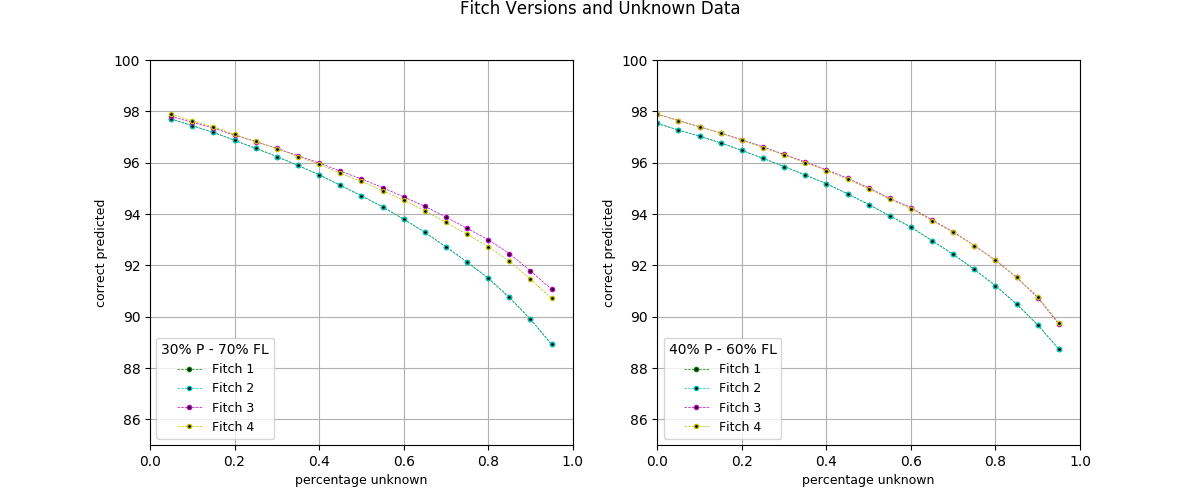
\includegraphics[width=0.8\textwidth]{Figures/simulation_fitch_evaluation.png}
          \caption{Test of Fitch Versions.}
          \label{fig:Fitch versions}
        \end{figure}
        These four versions were tested in the simulation with 100 trees and 10000 leaf nodes and a
          distribution of 60~\% FL to 40~\% P. Figure \ref{fig:Fitch versions} shows this over all unknown 
          node percentage. \\
        % At 90~\% unknown nodes and 90~\% of multifurcation of the internal nodes, version 1 was 89.26~\%, 
        %   version 2 was 89.26~\%, version 3 was 89.35~\%, and version 4 was 89.31~\% correct. Therefore, 
        %   only version 3 was used for all further simulations.
        At 95~\% unknown nodes and 95~\% of multifurcation of the internal nodes, version 1 was 88.37~\%, 
          version 2 was 88.37~\%, version 3 was 88.4~\%, and version 4 was 88.39~\% correct. Therefore, 
          only version 3 was used for all further simulations.
          
      % Fitch versions:
      % | 88.37 % | 88.37 % | 88.4 % |88.39 % |


      %---------------------------------------------------------------------------------------------------
      \subsubsection{Sankoff}
        Maximum parsimony algorithm from Sankoff implemented in the R package castor \cite{Louca2017}. \\
        \todo{transition probabilities: all equal}

  % %---------------------------------------------------------------------------------------------------
  % %---------------------------------------------------------------------------------------------------
  % %---------------------------------------------------------------------------------------------------
  % \section{real data analysis}
  %   \begin{itemize}
  %     \item Import tree
  %     \item Import interactions
  %     \item run castor algorithm / and others?
  %     \item interprete results (cross validation - leave 100 out)
  %   \end{itemize}

  %---------------------------------------------------------------------------------------------------
  %---------------------------------------------------------------------------------------------------
  %---------------------------------------------------------------------------------------------------
  \section{Implementation}
    \colorbox{red}{You} can find the full code on GitHub: 
      \hyperlink{github.com/Irallia/IZW-HU-Parasites}{github.com/Irallia/IZW-HU-Parasites}. \\
    Most of the code was written in Python. The analyzes and the use of the Castor package in R. There 
      are some shell scripts to execute whole workflows.

%---------------------------------------------------------------------------------------------------
%---------------------------------------------------------------------------------------------------
%---------------------------------------------------------------------------------------------------
%---------------------------------------------------------------------------------------------------
\chapter{Results}
  A big point in this chapter is the result of examining the input data. How is the situation? What 
    influence does that have on our actual result? What can we do about it? Our simulation gave us 
    some results to this. \\
  Otherwise, this chapter is mainly about the actual reconstruction of the states. This means, on 
    one hand investigation of origins and losses of the inner nodes and on the other, the prediction 
    of unknown states of leaf nodes. \\
   
  %---------------------------------------------------------------------------------------------------
  %---------------------------------------------------------------------------------------------------
  %---------------------------------------------------------------------------------------------------
  \section{Metadata analysis - Missing information}
    As previously presented, we have two types of missing information: unknown states of leaf nodes 
      and multifurcation. \\

    We examined the ridge of multifurcation of the tree. A complete phylogenetic tree would be 
      binary, which means the number of leaf nodes is closely to the number of internal nodes. But 
      since we only work with a synthesis tree, this tree is multifurcated: we have 241 974 internal 
      nodes and 2 293 463 leaf nodes. \\
    For a first overview we collected for every node its number of children (degree $-1$), and plotted
      this in two histograms, see figure \ref{fig:childrenOfNodes}. \\
    The multifurcation affects only the internal nodes. We collected the number of children $-2$ of 
      every node (a node with two children is binary). That means it discribes the number of nodes which we have lost from the real (binary) 
    phylogenetic tree. \\
    \begin{figure}[h!]
      \centering
      \begin{subfigure}[b]{0.5\textwidth}
        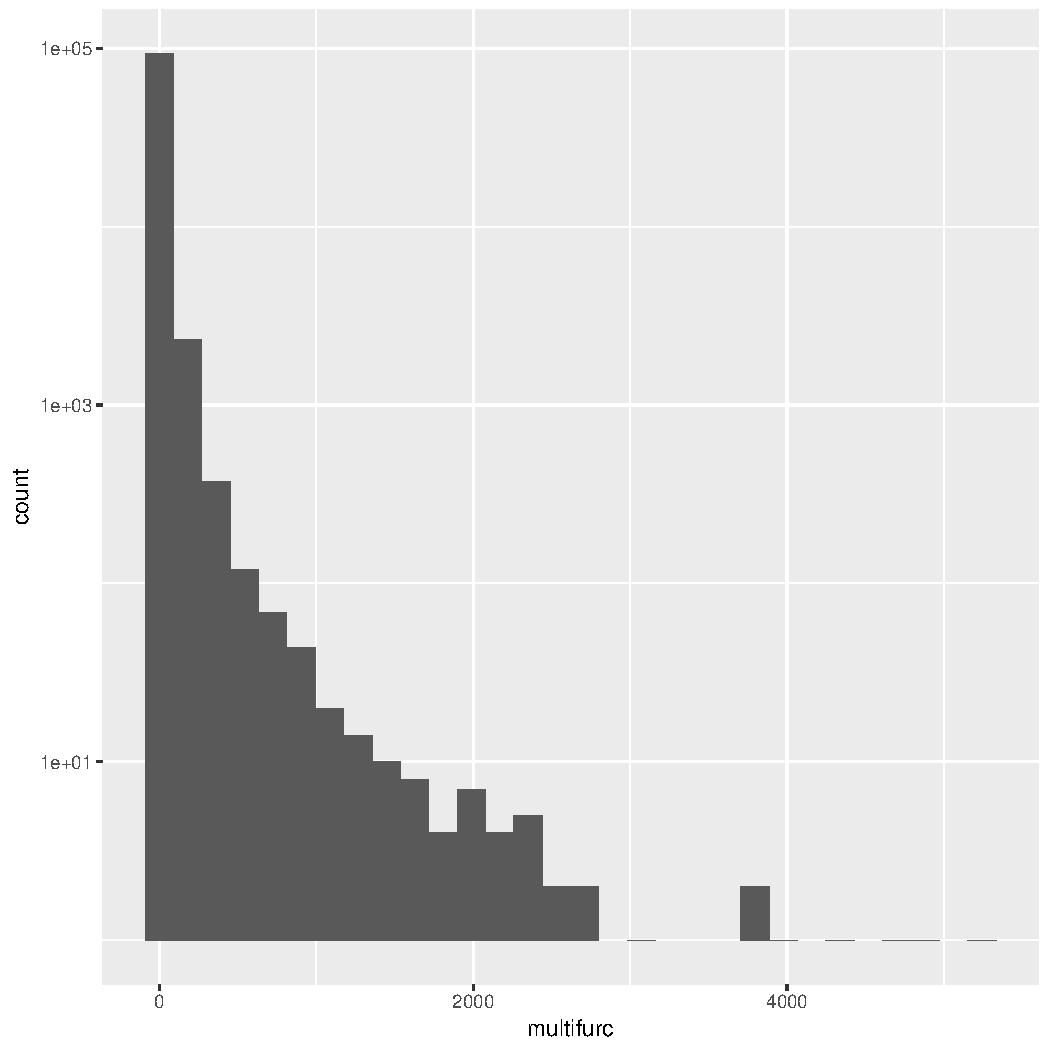
\includegraphics[width=0.9\textwidth]{Figures/multifurc.pdf}
        \caption{Histogram with automatic binwidth. \\ ~ \\ ~}
      \end{subfigure}
      ~~~ %add desired spacing between images, e. g. ~, \quad, \qquad, \hfill etc. 
        %(or a blank line to force the subfigure onto a new line)
      \begin{subfigure}[b]{0.42\textwidth}
        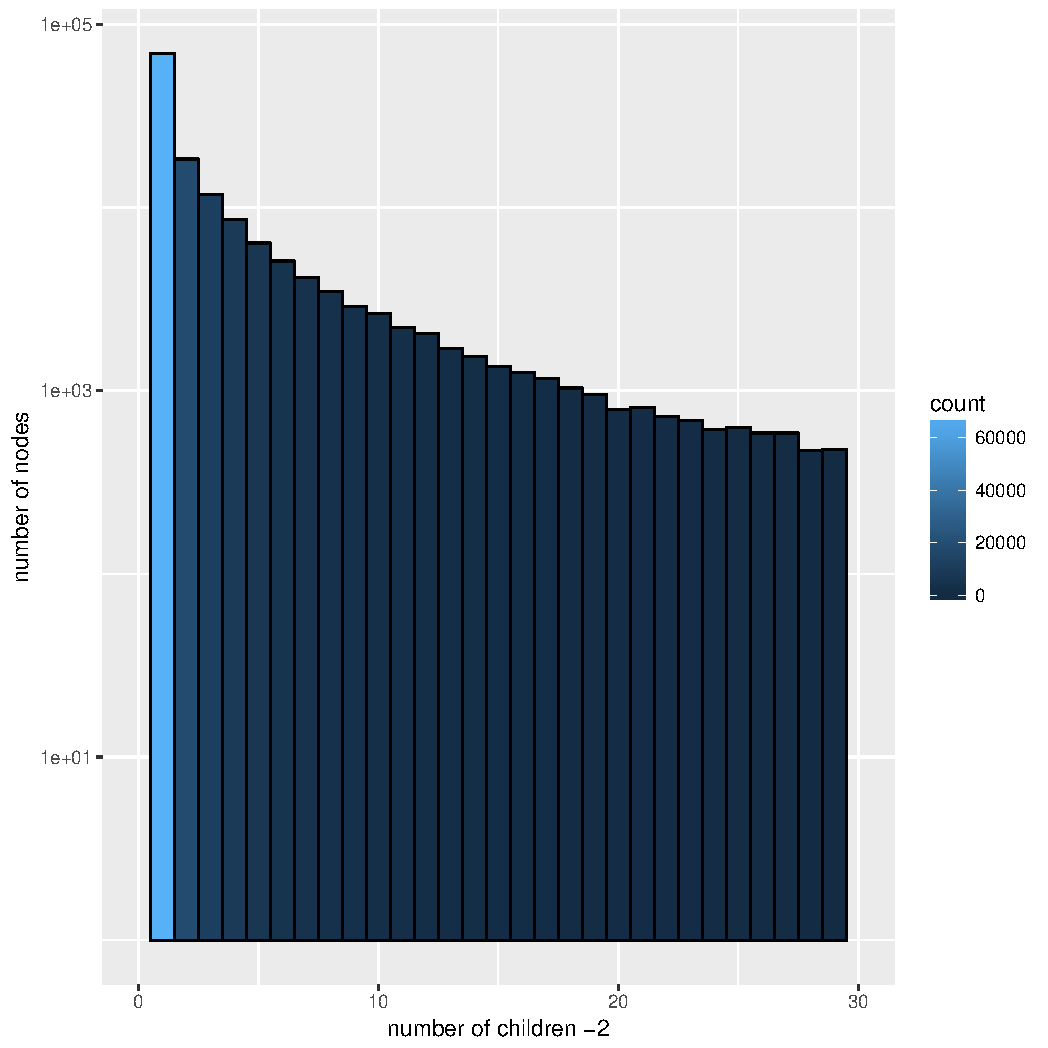
\includegraphics[trim = 0mm 0mm 30mm 0mm, clip, width=0.9\textwidth]{Figures/multifurc_small.pdf}
        \caption{Histogram with $binwidth = 1$. \\ light blue: binary; \\ dark blue: multifunction}
      \end{subfigure}
      \caption{Histograms about the multifurcation of the internal nodes of the synthesis tree.}
      \label{fig:childrenOfNodes}
    \end{figure}
    As \colorbox{red}{you} can see, we are very far from a binary tree. \\
    Some subtrees have been examined, these have the following percentages of missing information: See 
      table \ref{table:percentage loss information subtrees}.
    \begin{table}[h!]
      \begin{center}
        \begin{tabular}{ |l||r|r| }
          \hline
          Subtree of & unknown states & multifurcation \\ 
          \hline \hline
          Eukaryota       & 97.34~\%  & 98.16~\% \\
          \hline \hline
          Metazoa         & 96.44~\%  & 87.93~\% \\ \hline
          Fungi           & 98.87~\%  & 96.97~\% \\ \hline
          Chloroplastida  & 99.14~\%  & 89.46~\% \\
          \hline \hline            
          % Arthropoda      & 97.49~\%  & 89.95~\% \\ \hline
          Apicomplexa     & 86.26~\%  & 87.16~\% \\ \hline
          Nematoda        & 89.01~\%  & 88.59~\% \\ \hline
          Chordata        & 88.59~\%  & \cellcolor{green!50}66.49~\% \\ \hline
          Platyhelminthes & \cellcolor{green!50}68.73~\%  & 80.34~\% \\
          \hline \hline            
          Insecta         & 97.11~\%  & 90.78~\% \\
          \hline  
        \end{tabular}
      \end{center}
      \caption{Examination of subtrees regarding missing information. \\ 
        % Taxa of subtrees: Domain, Kingdom, Phylum, Class \\ 
        Unknown states: missing state information of leaf nodes \\ 
        Multifurcation: missing internal nodes}
      \label{table:percentage loss information subtrees} 
    \end{table}

    %---------------------------------------------------------------------------------------------------
    %---------------------------------------------------------------------------------------------------
    \subsection{Data artifacts}
      At this point we also found out that there are some nodes with only one child node (55,700 nodes). \\
      These are both, the most nodes are right in front of a leaf, as well as some nodes are deep in the 
        tree (3,956 with height $>2$). They are probably a result from the fact that taxonomic information 
        has been incorporated into a phylogeny. \\
      Some examples:
      \begin{itemize}
        \item Nephroselmidophyceae: (class) \\
          https://tree.opentreeoflife.org/opentree/argus/ottol@1038762
        \item Phrynocrinidae: (family) \\
          https://tree.opentreeoflife.org/opentree/argus/ottol@3647979
        \item Elaeocarpus sylvestris: \\
          https://tree.opentreeoflife.org/opentree/argus/opentree9.1@ott166969
      \end{itemize}

    %---------------------------------------------------------------------------------------------------
    %---------------------------------------------------------------------------------------------------
    \subsection{Taxa}
      The investigation of the taxonomy revealed that our tree has three kingdoms: Chloroplastida, 
        Metazoa, Fungi, 53 phyla, 195 classes and 924 orders. \\
      Since the analysis of the tree is not part of this work, it should be mentioned here that, 
        according to recent findings, this is not complete and we lack some taxa in every rank. For 
        example, Cavalier-Smith says that one distinguishes between seven and nine kingdoms 
        \cite{CavalierSmith1981}. \\
      In section \pageref{subsec:listPhyla} of the appendix \colorbox{red}{you} can find a list of all phyla.

    %---------------------------------------------------------------------------------------------------
    %---------------------------------------------------------------------------------------------------
    \subsection{Poisson regression of the multifurcation}
      First of all we measured the strength of the multifurcation with the help of the intercept: 
        $2.821 > 0$ $\Rightarrow$ there is a multifunction. \\
      Comparing the different kingdoms, we find that multifunctionality is greater in Fungi than in 
        Chloroplastida than in Metazoa:
      $$4.0999 (Fungi Intercept) > -0.9132 (Chloroplastida Intercept) > -1.4320 (Metazoa Intercept)$$
      % Degrees of Freedom: 96010 Total (i.e. Null);  96010 Residual
      Then we have 9 times 4 models of different complexity levels.
      \begin{table}[h!]
        \begin{center}
            \begin{tabular}{ |l|r|r|r|r| }
              \hline
              Model / Taxa & Kingdom & Phylum & Class & Order \\
              \hline \hline
              multifurc $\sim$ taxa & 7774454 & \cellcolor{green!10}7435700 & \cellcolor{green!15}7337241 & \cellcolor{green!30}7076068 \\
              \hline
              multifurc $\sim$ taxa + depth & 7752303 & \cellcolor{green!10}7431609 & \cellcolor{green!15}7334754 & \cellcolor{green!30}7027578 \\
              multifurc $\sim$ taxa + max.height & 7730196 & \cellcolor{green!15}7375889 & \cellcolor{green!20}7275856 & \cellcolor{green!30}7005424 \\
              multifurc $\sim$ taxa + min.height & \cellcolor{green!10}7472500 & \cellcolor{green!20}7233486 & \cellcolor{green!25}7144686 & \cellcolor{green!40}6890703 \\
              multifurc $\sim$ taxa + mean.height & \cellcolor{green!15}7304402 & \cellcolor{green!25}7128318 & \cellcolor{green!30}7055313 & \cellcolor{green!40}6815271 \\
              \hline
              multifurc $\sim$ taxa * depth & 7714881 & \cellcolor{green!15}7335396 & \cellcolor{green!20}7250759 & \cellcolor{green!40}6843004 \\
              multifurc $\sim$ taxa * max.height & \cellcolor{green!5}7692980 & \cellcolor{green!15}7311241 & \cellcolor{green!25}7187504 & \cellcolor{green!45}6795823 \\
              multifurc $\sim$ taxa * min.height & \cellcolor{green!10}7442387 & \cellcolor{green!25}7177002 & \cellcolor{green!30}7094933 & \cellcolor{green!45}6795099 \\
              multifurc $\sim$ taxa * mean.height & \cellcolor{green!20}7247309 & \cellcolor{green!30}7020258 & \cellcolor{green!35}6965794 & \cellcolor{green!50}6665565 \\
              \hline
            \end{tabular}
        \end{center}
        \caption{Residuals of multifurcation models}
        \label{table:Residuals multifurcation} 
      \end{table}
      In Table \ref{table:Residuals multifurcation} is a deviance table, where the different residuals 
        are listed. Since only residuals are comparable in complexity, we have also calculated the BIC 
        values of the models in table \ref{table:BIC multifurcation}. \\
      \begin{table}[h]
        \begin{center}
          \begin{tabular}{ |l|r|r|r|r| }
            \hline
            Model / Taxa & Kingdom & Phylum & Class & Order \\
            \hline \hline
            multifurc $\sim$ taxa & 8273333 & \cellcolor{green!15}7937828 & \cellcolor{green!20}7842157 & \cellcolor{green!30}7644249 \\
            multifurc $\sim$ taxa & 8257680 & \cellcolor{green!15}7922207 & \cellcolor{green!20}7826490 & \cellcolor{green!35}7574154 \\
            \hline
            multifurc $\sim$ taxa + depth & 8273318 & \cellcolor{green!15}7934322 & \cellcolor{green!20}7839364 & \cellcolor{green!35}7539999 \\
            multifurc $\sim$ taxa + max.height & \cellcolor{green!15}7993515 & \cellcolor{green!25}7749121 & \cellcolor{green!30}7661817 & \cellcolor{green!40}7416211 \\
            multifurc $\sim$ taxa + min.height & 8251211 & \cellcolor{green!20}7875521  & \cellcolor{green!25}7778327 & \cellcolor{green!35}7516883 \\
            multifurc $\sim$ taxa + mean.height & \cellcolor{green!20}7825417 & \cellcolor{green!30}7644249 & \cellcolor{green!35}7572474 & \cellcolor{green!45}7340741 \\
            \hline
            multifurc $\sim$ taxa * depth & 8235932 & \cellcolor{green!20}7836755 & \cellcolor{green!25}7757688 & \cellcolor{green!45}7383808 \\
            multifurc $\sim$ taxa * max.height & \cellcolor{green!15}7963438 & \cellcolor{green!30}7693555 & \cellcolor{green!30}7614820 & \cellcolor{green!45}7335338 \\
            multifurc $\sim$ taxa * min.height & 8214030 & \cellcolor{green!20}7808940 & \cellcolor{green!30}7690618 & \cellcolor{green!45}7336627\\
            multifurc $\sim$ taxa * mean.height & \cellcolor{green!25}7768360 & \cellcolor{green!35}7536296 & \cellcolor{green!50}7484953 & \cellcolor{green!50}7206369 \\
            \hline
          \end{tabular} 
        \end{center}
        \caption{BIC of multifurcation models}
        \label{table:BIC multifurcation} 
      \end{table}
      % * Residuals: Fehler - wieviele Werte sind nicht gut modelliert. (umso kleiner umso besser - grün) \\
      The Residuals give us the error of the model. If the value is small, our data will be well modeled. \\
      Within the complexity classes it can be seen that the mean height gives the best additional factor. \\
      
      Despite higher complexity, the BIC values are getting smaller from model to model, meaning that 
        the finest model available here is also the best one of these. Smaller taxa than orders (eg 
        family) were computationally too expensive to calculate.

    %---------------------------------------------------------------------------------------------------
    %---------------------------------------------------------------------------------------------------
    \subsection{Binomial regression of the unknown state information}

      Next to the problem of the multifurcation of the tree is the less of data we have for the species.
        For the ancestral state reconstruction, we need information in the leaf nodes. \\
      The eukaryotic synthesis tree has 293,463 leaf nodes. The GloBI database has 5 346 414 interactions 
        (at this timepoint). Out of this data we got 51,337 distinct free-living species and 47 332 
        distinct parasite species $\rightarrow$ unknown nodes 2,194,794 ($\approx 95.7~\%$). \\
      We found also 57,352 (not distinct!) source species and 809,993 (not distinct!) target
        species without OTT ids. Since we currently use only OTT ids, we could not use this information. \\
      % \todo{With this only $\approx 4.3~\%$ information in our leaf nodes are ...} \\

      We also compared different models in terms of their BICs (Table: \ref{table:BIC unknown information}). 
        The Residuals are not very meaningful here, since all models have different complexities. % /dimensions
        For the sake of completeness, the associated deviance tables are located with the residuals in 
        the appendix \ref{sec:Residuals unknown information}.

      \begin{table}[h!]
        \begin{center}
          \begin{tabular}{ |l|r|r|r|r| }
            \hline
            Model / Taxa & Kingdom & Phylum & Class & Order \\
            \hline \hline
            multifurc $\sim$ taxa & \cellcolor{green!15}545799 & \cellcolor{green!35}500004 & \cellcolor{green!45}485121 & \cellcolor{green!45}484681 \\
            \hline
            multifurc $\sim$ taxa + depth & \cellcolor{green!15}544862 & \cellcolor{green!40}493808 & \cellcolor{green!45}481869 & \cellcolor{green!50}478851 \\
            \hline
            multifurc $\sim$ taxa * depth & \cellcolor{green!15}544179 & \cellcolor{green!45}489845 & \cellcolor{green!45}481494 & \cellcolor{green!50}478188 \\
            \hline
          \end{tabular} 
        \end{center}
        \caption{BICs of unknown information}
        \label{table:BIC unknown information} 
      \end{table}
      It also follows from this table that the most complex model is the best. In general, the BIC 
        values are smaller than those of the multifurcation models. The modeling here is thus better. \\
      Again, the calculation of finer models (eg order or family) was too expensive. \\

      These missing data modeling results can be used to better simulate the data.

  %---------------------------------------------------------------------------------------------------
  %---------------------------------------------------------------------------------------------------
  %---------------------------------------------------------------------------------------------------
  \section{Results of simulation / Influence of different parameters}

    As presented, we compare two methods in our simulation to their prediction accuracy: Fitch and 
      Sankoff. \\
    We examine different parameters. In figure \ref{fig:influence of unknown data} is an overview of 
      the results. \\
    The first column describes the distributions of free-livings and parasites with a given threshold 
      for the respective simulations to the right. \\
    The middle column investigates the influence of the unknown states, the right the influence of the 
      strength of the multifurcation. \\
    The y-axes indicate the percentage of correctly predicted states (including known states). On the 
      x-axis the percentage of forgotten states or missing internal nodes. \\
    Each point corresponds to the average of one hundred simulations, each with 10,000 leaf nodes. \\
    For the middle column we set the strength of the multifurcations to 0.95~\% similar to the real 
      data and in the right column the amount of the unknowns to 0.95~\% also similar to the real data. \\

    As \colorbox{red}{you} can see both algortithms are always over 50~\% and therefore better than guessing. Moreover, 
      they are usually close to each other, with Sankoff always makes better predictions except for 
      equally distributed states as Fitch. \\
    \colorbox{red}{You} can see that the distribution of states has a strong influence on the prediction. The more 
      evenly distributed, the harder it is to predict. \\
    If more than 60~\% of internal nodes are missing, Fitch breaks significantly in his prediction 
      compared to Sankoff.
    
    \begin{figure}
      \centering
      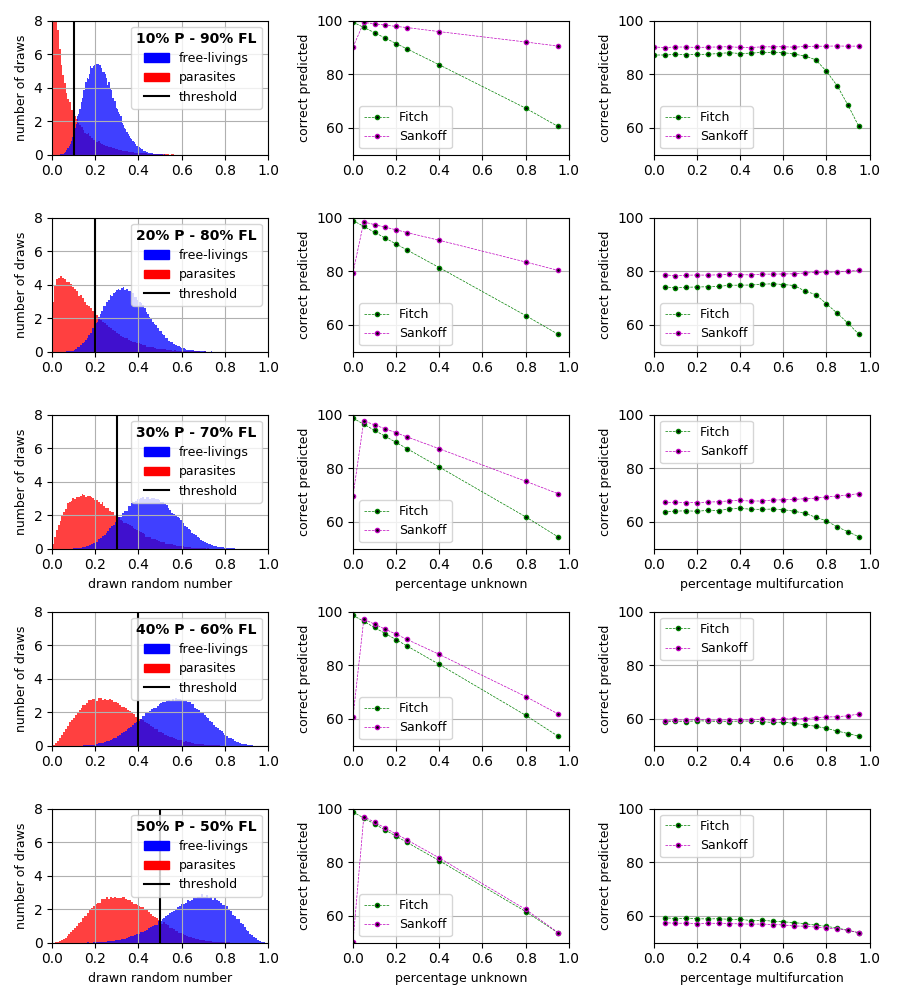
\includegraphics[trim = 0mm 0mm 0mm 0mm, clip, width=\textwidth]{Figures/simulation_evaluation_1.png}
      \caption{Influence of unknown data to prediction}
      \label{fig:influence of unknown data}
    \end{figure}

    In the end, Sankoff is in most cases the more accurate algortihmus and was therefore used for our 
      prediction of the real data.

  %---------------------------------------------------------------------------------------------------
  %---------------------------------------------------------------------------------------------------
  %---------------------------------------------------------------------------------------------------
  \section{Results of the real data analysis created with Sankoff}

    %---------------------------------------------------------------------------------------------------
    %---------------------------------------------------------------------------------------------------
    \subsection{Biological view}
      To analyze the results, we have selected some phyla (sub-trees) to evaluate our results 
        selectively from the biological point of view: Chordata, Nematoda, Platyhelminthes and 
        Apicomplexa. \\
      In Table \ref{table:phylum leaf nodes states} we compare the given states with the predicted ones. \\
      There are several factors that play a role here, and in part, crystallize in these examples. \\
      An important factor here is that the credibility of the results with the accuracy of the input 
        data, i. the data of GloBI, stands and falls. Errors of incorrect input data can be amplified by 
        incorrect prediction of unknown species and can be reversed in order to improve the data 
        situation of GloBI. \\
      Since we look at such large trees we can not expect to know all the parasites, so we look at 
        individual positives. Positive in the sense that the majority have the opposite state.

      \begin{table}[h]
        \begin{center}
          \begin{tabular}{ |l|r||r|r||r|r|r|r| }
            \hline
            & & \multicolumn{2}{c||}{original states} & \multicolumn{4}{c|}{final states} \\
            Phylum & \# nodes       & FL & P              & 0 (FL) & 0.3 & 0.5 & 1 (P) \\
            \hline \hline
            Chordata & 91785        & 10451 & 18          & 91759 & 0 & 0 & 26 \\
            &                       & 99.83~\% & 0.49~\%  & 99.97~\% & & & 0.03~\% \\ \hline
            Nematoda & 30127        & 21 & 3289           & 1604 & 142 & 1196 & 27185 \\
            &                       & 0.63~\% & 99.37~\%  & 5.32~\% & 0.47~\% & 3.97~\% & 90.23~\% \\ \hline
            Platyhelminthes & 22683 & 7 & 7086            & 175 & & & 22508 \\
            &                       & 0.1~\% & 99.9~\%    & 0.77~\% & 0 & 0 & 99.23~\% \\ \hline
            Apicomplexa & 1863      & 1 & 255             & 1 & 0 & 0 & 1862 \\
            &                       & 0.39~\% & 99.61~\%  & 0.05~\% & & & 99.95~\% \\
            % \hline \hline
            % Phylum & \# nodes & FL & P
            %   & 0 (FL) & 0.4 & 0.5 & 0.67 & 0.75 & 1 (P) \\
            % Arthropoda & 1198981 & 18912 & 11141 
            %   & 1099509 & 1313 & 22478 & 4176 & 1665 & 70223 \\
            % & & 62.93~\% & 37.07~\%
            %   & 91.7~\% & 0.11~\% & 1.87~\% & 0.35~\% & 0.14~\% & 5.86~\% \\
            \hline
          \end{tabular} 
        \end{center}
        \caption{Phylum (leaf nodes)}
        \label{table:phylum leaf nodes states} 
      \end{table}

      In contrast to the other phyla examined, the phylogeny is more pronounced (less multifurcation) (see 
        Table \ref{table:percentage loss information subtrees}). This results in a weaker spread of errors. 
        This is reflected in the results from the table \ref{table:phylum leaf nodes states}. There are 18 
        parasites as input data and only 8 more are predicted. The chordata mostly consist of free-living 
        species, so this seems believable. We started with 99.83~\%  species and predict 99.97~\% species 
        as free-living (including already known nodes). \todo{A few punctual tests give us the following:}

      \begin{figure}[h!]
        \centering
        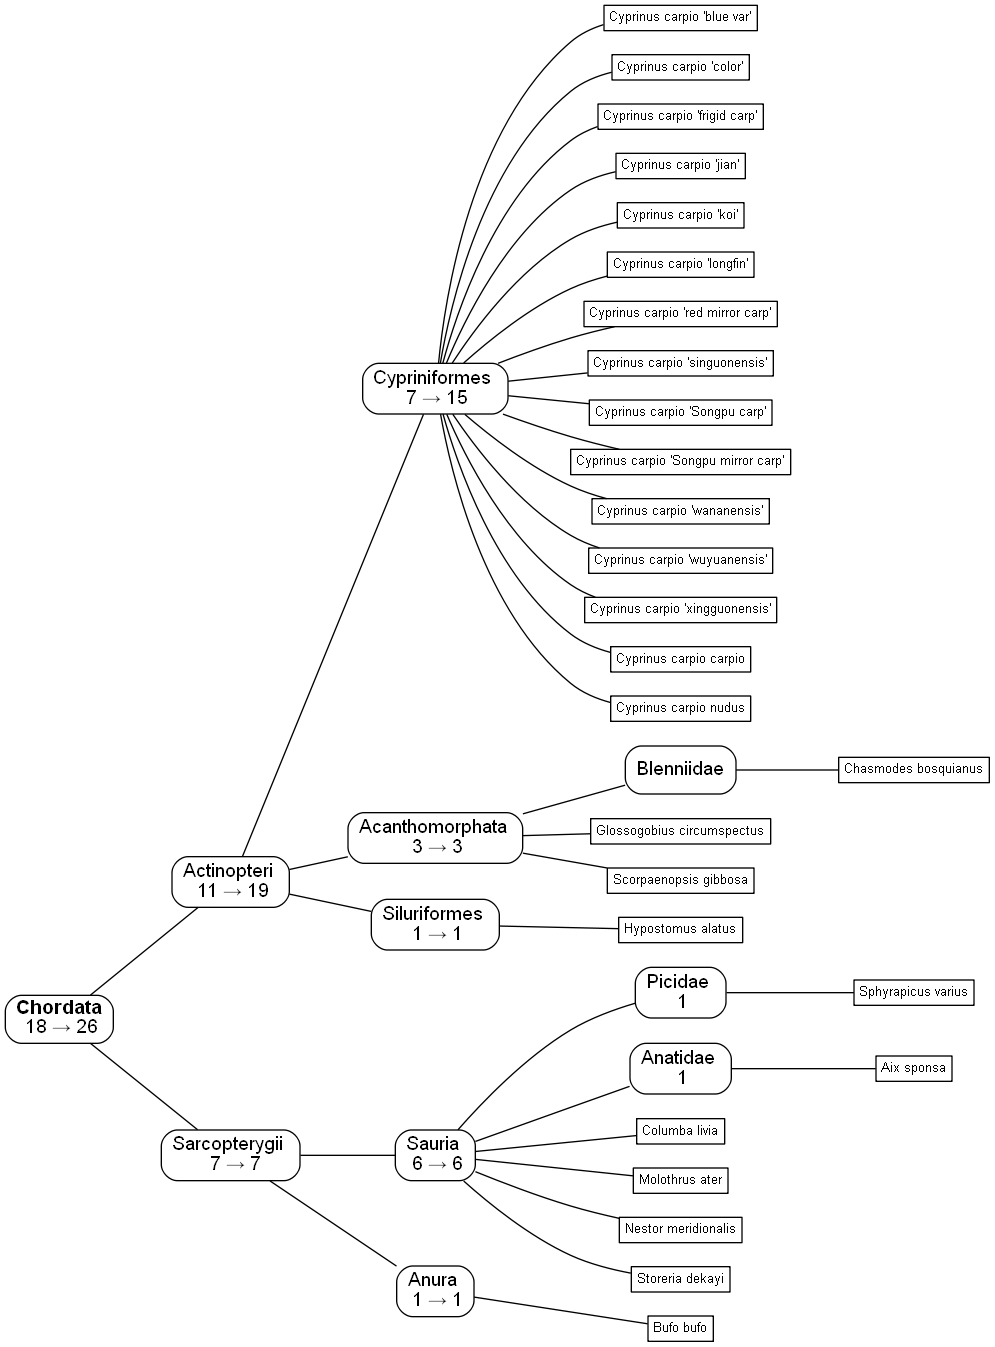
\includegraphics[trim = 0mm 0mm 0mm 0mm, clip, width=0.85\textwidth]{Figures/ChordataParasites.png}
        \caption{Parasites of Phylum: Chordata \\ 
          Input parasites (green) $\rightarrow$ predicted parasites (white $\rightarrow$ green)}
        \label{fig:ChordataParasites}
      \end{figure}

      We mapped the few parasitic spezies in a rough taxonomy (see Figure \ref{fig:ChordataParasites}): \\
      Known parasitic birds belong to the order Sauria. Here we know from Rothschild  here there are 
        breeding parasites, like the cuckoo and clepto-parasites as the skuas \cite{Rothschild1957}. We
        got 6 input parasites from GloBI and there are no predictions: A woodpecker - 
        \textit{Sphyrapicus varius} and a duck - \textit{Aix sponsa}, a cow bird - \textit{Molothrus ate} 
        known as broodparasite and some others. \\
      An example of the amplification of mistakes here are the carp. There seems to be a paper from the 
        GloBI concluding: Grass carp (\textit{Ctenopharyngodon idella)} has Pathogen common carp 
        (\textit{Cyprinus carpio})\footnote{
          \hyperlink{https://www.globalbioticinteractions.org/?interactionType=hasParasite&targetTaxon=Cyprinus\%20carpio}
          {https://www.globalbioticinteractions.org/?interactionType=hasParasite\&targetTaxon=Cyprinus\%20carpio}
        }. Since there is hardly any information about free-living, it follows that all siblings are 
        also predicted to be parasitic. \\
        % Other birds: Columba livia, Nestor meridionalis, Sphyrapicus varius \\
        % Snake: Storeria dekayi (probably caused by wrong input data.)
      % \begin{itemize}
      %   \item Order Acanthomorphata(3):, one slime fish (family Blenniidae) and two others without family
      %   \item Order Anura (1): a toad (Family Bufonidae) - there exists some parasitic species in here, 
      %     they eat fin or pieces of larger fish.
      %   \item Order Siluriformes (1): a catfish (Family Loricariidae) - there exists some parasitic 
      %     species in here.
      % \end{itemize}

      The Apicomplexa are a parasitic phylum. We found only one input organism: Stemonitis fusca as a 
        free-living specie. In GloBI it is listed as being parasitized by Nectria candicans and Nectriopsis 
        sporangiicola\footnote{
          \hyperlink{https://www.globalbioticinteractions.org/?interactionType=parasiteOf&targetTaxon=Stemonitis\%20fusca}
          {https://www.globalbioticinteractions.org/?interactionType=parasiteOf\&targetTaxon=Stemonitis\%20fusca}
        }. The algorithm has not predicted new free-livings. \\

      Most species of Platyhelminthes (flatworms) are parasites, although there are also free-living, 
        predatory feeding species. These are summarized in the Turbellaria, while the parasites are 
        divided into three other classes \cite{Ax1961}. This also corresponds to our observations. There 
        is one class (Rhabditophora) that contains all but one single exception of free-living species 
        of this phylum, which includes the Turbellaria. \\
      It should be noted, however, that this classification is outdated, as it has been proven that 
        the Turbellaria are not monophyletic. But we will not go into that here. \\
      For the Platyhelminthes we had more state information for the leaf nodes compared to the other 
        considered subtrees, see Table \ref{table:percentage loss information subtrees}. We start with 
        0.1~\% free-livings and predicted 0.77~\% as free-living spezies. \\
    %---------------------------------------------------------------------------------------------------

      With the Nematoda it looks more complicated. Large parts of Nematoda are free-living, but we 
        found only 5.32~\% of them. Blaxter et al. estimates the order of 25,000 parasites in the 
        Nematoda \cite{Blaxter2015} and speaks of at least seven independently arosed parasitism 
        \cite{Blaxter1998}. In a recent article Blaxter identifies 18 origins \cite{Blaxter2015} in 
        Nematoda. \\
      The problem at this point, however, is obvious: Hallan speaks of the fact that only 23,00 species 
        were described by the Nematoda but one assumes 1 million or more\footnote{J. Hallan, unpublished; 
          \hyperlink{https://insects.tamu.edu/research/collection/hallan/}
          {https://insects.tamu.edu/research/collection/hallan/}
        }. \todo{Link ist nicht erreichbar!} The parasites have been much more studied and thus we start 
        with only 0.63~\% free-living species. Against such a shifted data situation, the algorithm is 
        almost powerless. And yet the percentage has increased. \\

      % \anmerkungstext{Das sind schonmal vier große Kontraste, wenn dann noch Zeit bleibt, die 
      %   schwirigen... Arthropoden, Fungi, Pflanzen... (Emanuel)} \\

      \todotext{Im Folgenden folgen 3 weitere ähnliche tabellen. Einmal eine ähnliche Tabelle inklusive 
        interner Knoten \ref{table:Phylum internal nodes}, zweimal die Übersicht über die Kingdoms 
        Blattknoten \ref{table:Kingdom leaf nodes} bzw interne Knoten \ref{table:Kingdom internal nodes}. Welche 
        nehmen wir? Rest Appendix oder ganz raus?}

      \begin{table}[h!]
        \begin{center}
          \begin{tabular}{ |l|r||r|r||r|r|r|r|r|r| }
            \hline
            & & \multicolumn{2}{c||}{original states} & \multicolumn{6}{c|}{final states} \\
            Phylum & \# nodes & FL & P
              & 0 (FL) & 0.4 & 0.5 & 0.67 & 0.75 & 1 (P) \\
            \hline \hline
            Chordata & 122546 & 10451 & 18 
              & 122473 & 0 & 0 & 0 & 0 & 73 \\
            Nematoda & 33564 & 21 & 3289 
              & 846 & 0 & 1133 & 0 & 0 & 31585 \\
            Platyhelminthes & 27142 & 7 & 7086 
              & 1010 & 0 & 175 & 0 & 0 & 25957 \\
            Apicomplexa & 2102 & 1 & 255 
              & 1 & 0 & 0 & 0 & 0 & 2101 \\
            % \hline
            % Arthropoda & 1319460 & 18912 & 11141 
            %   & 1207204 & 1313 & 25499 & 4852 & 1957 & 78635 \\
            \hline
          \end{tabular}
        \end{center}
        \caption{Phylum (inkl internal nodes)}
        \label{table:Phylum internal nodes}
      \end{table}

      \begin{table}[h!]
        \begin{center}
          \hspace*{-2cm}\begin{tabular}{ |l|r||r|r||r|r|r|r|r|r|r|r| }
            \hline
            & & \multicolumn{2}{c||}{original states} & \multicolumn{8}{c|}{final states} \\
            Kingdom & \# nodes & FL & P
              & 0 (FL) & 0.25 & 0.33 & 0.4 & 0.5 & 0.67 & 0.75 & 1 (P) \\
            \hline \hline
            none & 75446 & 45 & 529 
              & 13426 & 220 & 24082 & 0 & 7792 & 5302 & 0 & 24493 \\
            Fungi & 31457 & 577 & 2983
              & 38520 & 0 & 0 & 0 & 5723 & 0 & 0 & 266463 \\
            Chloroplastida & 416478 & 3519 & 77
              & 410795 & 0 & 0 & 0 & 4182 & 0 & 0 & 1501 \\
            Metazoa & 1491012 & 30758 & 22373
              & 1328135 & 0 & 0 & 930 & 25535 & 4423 & 1665 & 130324 \\
            \hline  
          \end{tabular}
        \end{center}
        \caption{Kingdom (leaf nodes)}
        \label{table:Kingdom leaf nodes}
      \end{table}

      \begin{table}[h!]
        \begin{center}
          \hspace*{-2cm}\begin{tabular}{ |l|r||r|r||r|r|r|r|r|r|r|r| }
            \hline
            & & \multicolumn{2}{c||}{original states} & \multicolumn{8}{c|}{final states} \\
            Kingdom & \# nodes & FL & P
              & 0 (FL) & 0.25 & 0.33 & 0.4 & 0.5 & 0.67 & 0.75 & 1 (P) \\
            \hline \hline
            none & 84456 & 45 & 529 
              & 15035 & 243 & 25910 & 0 & 8764 & 6183 & 0 & 28140 \\
            Fungi & 324105 & 577 & 2983
              & 39088 & 0 & 0 & 0 & 5858 & 0 & 0 & 274803 \\
            Chloroplastida & 460457 & 3519 & 77
              & 454211 & 0 & 0 & 0 & 4688 & 0 & 0 & 1558 \\
            Metazoa & 1670956 & 30758 & 22373
              & 1485749 & 0 & 0 & 1313 & 29002 & 5102 & 1957 & 147833 \\
            \hline  
          \end{tabular}
        \end{center}
        \caption{Kingdom (inkl internal nodes)}
        \label{table:Kingdom internal nodes}
      \end{table}


    %---------------------------------------------------------------------------------------------------
    %---------------------------------------------------------------------------------------------------
    \subsection{Origins and Losses}

      Weinstein and Kuris have been searching for origins of parasitism in Animalia \cite{Weinstein2016}. 
        They identified 223 parasitic origins: 223 in Metazoa $\supset$ 143 in Arthropoda $\supset$ 87 
        in Insecta. \\
      This has led us to count the origins and losses of parasitism in our investigation as well. \\
      We count only one origin / loss in a parent node with different children's nodes. \\
      Here we have encountered a problem: The Castor algorithm gives us probabilities for states. That 
        means there are also nodes with state like 0.3 or 0.5. So how do \colorbox{red}{you} count? Our solution was, 
        to round these values. We have to say that we round 0.5 to 0.

      \begin{table} [h]
        \begin{center}
          \begin{tabular}{ |l|r|r||r|r|r| }
            \hline
            Domain  & \# internal & \# leaf & Rootnode & \multicolumn{2}{c|}{without and with rounding} \\ 
            / Kingdom  & \multicolumn{2}{c||}{nodes} & state & \# origins & \# losses \\
            / Phylum / Class & & & & (FL -> P) & (P -> FL) \\
            \hline \hline
            Eukaryota & 241974 & 2293463 & 1.0 & 415 & 363 \\
            & & & P & 462 & 369 \\
            \hline \hline
            Metazoa & 179944 & 1491012 & 0.5 & 294 & 123 \\
            & & & & 321 & 129 \\ \hline
            Fungi & 9534 & 314571 & 0.5 & 80 & 222 \\
            & & & & 97 & 222 \\ \hline
            Chloroplastida & 43486 & 412434 & 0.0 & 40 & 2 \\
            & & & FL & 42 & 2 \\
            \hline \hline            
            Arthropoda & 120479 & 1198981 & 0.0 & 260 & 102 \\
            & & & FL & 281 & 108 \\ \hline
            Apicomplexa & 239 & 1863 & 1.0 & 0 & 1 \\
            & & & P & 0 & 1 \\ \hline
            Nematoda & 3437 & 30127 & 1.0 & 0 & 11 \\
            & & & P & 2 & 11 \\ \hline
            Chordata & 30761 & 91785 & 0.0 & 12 & 1 \\
            & & & FL & 12 & 1 \\ \hline
            Platyhelminthes & 4459 & 22683 & 1.0 & 0 & 5 \\
            & & & P & 0 & 5 \\
            \hline \hline            
            Insecta & 91256 & 989572 & 0.0 & 234 & 77 \\
            & & & FL & 245 & 77 \\ 
            \hline  
          \end{tabular}
        \end{center}
        \caption{Origins and losses}
        \label{table:origins and losses} 
      \end{table}

      In Table \ref{table:origins and losses} we can see, that we found some more origins than Weinstein 
        and on top of that some losses. \\
      
      Lets have a look at the same phyla as in the section before: Chordata, Nematoda, 
        Platyhelminthes and Apicomplexa. \\
      Chordata are full of free-living species and so we see only a few origins of parasitism. The root
      and mostly all species are predicted as free-living. \\
      In Apicomplexa and the Platyhelminthes are looking fine too. Our algorithm gives us only one loss 
        of parasitism in Apicomplexa and five in the Platyhelminthes. They are both from the root over 
        mostly all species predicted as parasites. \\
      Nematoda is again full of problems. The rootnode is predicted as a parasite and so we have more 
        losses of parasitism for the less information of free-living species in this phylum. The rest 
        is parasitic \\
        As we have already mentioned Blaxter et al. found at least seven origins of parasitism 
          \cite{Blaxter1998}. If we assume that the root node of Nematoda is free-living, then some 
          losses would have to turn around and become Origins. So it could be that we end up in a similar 
          size as Blaxter.

      \begin{lstlisting}[gobble=6]
        possible tags: 0, 0.333, 0.4, 0.5, 0.667, 0.75, 1
        rounded to:    0  0      0    0    1      1     1
      \end{lstlisting}

      % \begin{lstlisting}[gobble=6]
      %   # possible tags: 0, 0.333, 0.4, 0.5, 0.667, 0.75, 1
      %   # rounded to:    0  0      0    0    1      1     1
      %   if node_state != father_state:
      %     if father_state == 0:
      %         origins += 1        # FL -> P
      %         new_found = True
      %     else:
      %         losses += 1         # P -> FL
      %         new_found = True
      % \end{lstlisting}

      % \todo{without rounding change else: to elif $father_state == 1$}
      
    %---------------------------------------------------------------------------------------------------
    %---------------------------------------------------------------------------------------------------
    \subsection{Cross evaluation - leave 100 out}
      We ran the castor algorithm 100 times with leaving 100 randomized free-living or parasitic species 
        out of the input data to see how stable our result is. Of these 10,000 nodes, 9,238 were unique. 
        Of that, we predicted 9060 ($\approx 98.17~\%$) correctly and 169 ($\approx 1.82~\%$) wrongly, 
        with duplicate draws always having the same prediction. \\
      What is the best way to model this data? We again tested the influence of the taxa and the depth 
        of leaf nodes and calculated the BICs (Table: \ref{table:BIC cross validation}).

      \begin{table}[h]
        \begin{center}
          \begin{tabular}{ |l|r|r|r|r| }
            \hline
            Model / Taxa & Kingdom & Phylum & Class & Order \\
            \hline \hline
            correct predicted $\sim$ taxa & 117877 & 111466 & XXXXX & XXXXX \\
            \hline
            correct predicted $\sim$ taxa + depth & 117703 & XXXXX & XXXXX & XXXXX \\
            \hline
            correct predicted $\sim$ taxa * depth & 117592 & XXXXX & XXXXX & \cellcolor{green!60}XXXXX \\
            \hline
          \end{tabular} 
        \end{center}
        \caption{Residuals of cross validation prediction}
        \label{table:Residuals cross validation} 
      \end{table}

      \begin{table}[h]
        \begin{center}
          \begin{tabular}{ |l|r|r|r|r| }
            \hline
            Model / Taxa & Kingdom & Phylum & Class & Order \\
            \hline \hline
            correct predicted $\sim$ taxa & 117936 & 112242 & 111733 & XXXXX \\
            \hline
            correct predicted $\sim$ taxa + depth & 117776 & XXXXX & XXXXX & XXXXX \\
            \hline
            correct predicted $\sim$ taxa * depth & XXXXX & XXXXX & XXXXX & \cellcolor{green!60}XXXXX \\
            \hline
          \end{tabular} 
        \end{center}
        \caption{BICs of cross validation prediction}
        \label{table:BIC cross validation} 
      \end{table}

      What could happen by removing a parasite or free-living of the list?
      \begin{itemize}
        \item It could be a specie, which don't exist in the tree leaf nodes. -> no effect
        \item It could be a specie, which exists in both lists. -> If it was a parasite, it is now 
          free-living, because we prefer parasites. Otherwise we have no effect again. (1053 are possible)
        \item Normal case: We loose information, because its a specie in our tree and we change it to a 
          leave node with no information.
      \end{itemize}

      Influence on the rest of the data:
      \begin{table}
        \begin{center}
          \begin{tabular}{ |cl||r|r|r|r|r| }
            \hline
            & & min & max & mean & variance ($\sigma^2$) & $\sigma$ \\
            \hline \hline
            \multirow{3}{*}{distance} & all   & 0 & 3587.70 & 224.96 & 313650.61 & 560.05 \\
            & leaf nodes                      & 0 & 3021.12 & 208.69 & 248103.38 & 498.10 \\
            & internal nodes                  & 0 & 566.58 & 16.28 & 4927.95 & 70.20 \\ \hline
            \multicolumn{2}{|c||}{changed tag} & 0 & 0 & 0 & 0 & 0 \\ \hline
            \multirow{3}{*}{lost} & all tags  & 100 & 100 & 100 & 0 & 0 \\
            & FL tags                         & 44 & 66 & 57.25 & 19.50 & 4.42 \\
            & P tags                          & 34 & 56 & 42.75 & 19.50 & 4.42 \\
            \hline
          \end{tabular}
        \end{center}
        \caption{Statistics to Cross validation}
      \end{table}

      \begin{table}
        \begin{center}
          \begin{tabular}{ |cl||r|r|r|r| }
            \hline
            & & min & max & mean & variance \\
            \hline \hline
            \rowcolor{green!50}distance & all   & 1 & 2 & 1.33 & 0.33 \\
            \rowcolor{orange!50}&               & 0 & 3587.70 & 217.94 & 273760.68 \\
            \rowcolor{green!50}& leaf nodes     & 1 & 2 & 1.33 & 0.33 \\
            \rowcolor{orange!50}&               & 0 & 3021.12 & 202.57 & 209274.86 \\
            \rowcolor{green!50}& internal nodes& 0 & 0 & 0.00 & 0.00 \\
            \rowcolor{orange!50}&               & 0 & 566.58 & 15.37 & 5684.00 \\ \hline
            \rowcolor{green!50}lost & FL tags   & 44 & 49 & 46.67 & 6.33 \\
            \rowcolor{orange!50}&               & 51 & 66 & 57.95 & 13.47 \\
            \rowcolor{green!50}& P tags         & 51 & 56 & 53.33 & 6.33 \\
            \rowcolor{orange!50}&               & 34 & 49 & 42.05 & 13.47 \\
            \hline
          \end{tabular}
        \end{center}
        \caption{Statistics to Cross validation \\
          - \colorbox{green!50}{Less free-livings - 3 examples} \\
          - \colorbox{orange!50}{Less parasites - 64 examples}}
      \end{table}

  %---------------------------------------------------------------------------------------------------
  %---------------------------------------------------------------------------------------------------
  %---------------------------------------------------------------------------------------------------
  \section{Effects of Taxa in the different models}

    The comparisons of the effects of the taxa can be found in Table \ref{table:Effects unknown data} 
    and showed ...

    \begin{table}[h!]
      \begin{center}
        \begin{tabular}{ |l|l|r|r|r|r| }
          \hline
          Taxa & Model / Effects & min & max & mean & median \\
          \hline \hline
          Kingdom & globi $\sim$ taxa         & 0,01 & 0,04 & 0,02 & 0,01 \\
                  & globi $\sim$ taxa + depth & 0,01 & 0,03 & 0,02 & 0,01 \\
                  & globi $\sim$ taxa * depth & 0,00 & 0,03 & 0,01 & 0,01 \\
          \hline
          Phylum & globi $\sim$ taxa          & 0,17 & 393501,80 & 32208,79 & 6149,78 \\
                  & globi $\sim$ taxa + depth & 0,32 & 567010,90 & 55149,54 & 10783,18 \\
                  & globi $\sim$ taxa * depth & 0,00 & 1000000,00 & 225375,33 & 2511,58 \\
          \hline
        \end{tabular} 
      \end{center}
      \caption{Effects of Taxa in models for unknown data}
      \label{table:Effects unknown data} 
    \end{table}

    globi $\sim$ taxa * depth: NOTE: kingdom is not a high-order term in the model

    \begin{figure}[h!]
      \centering
      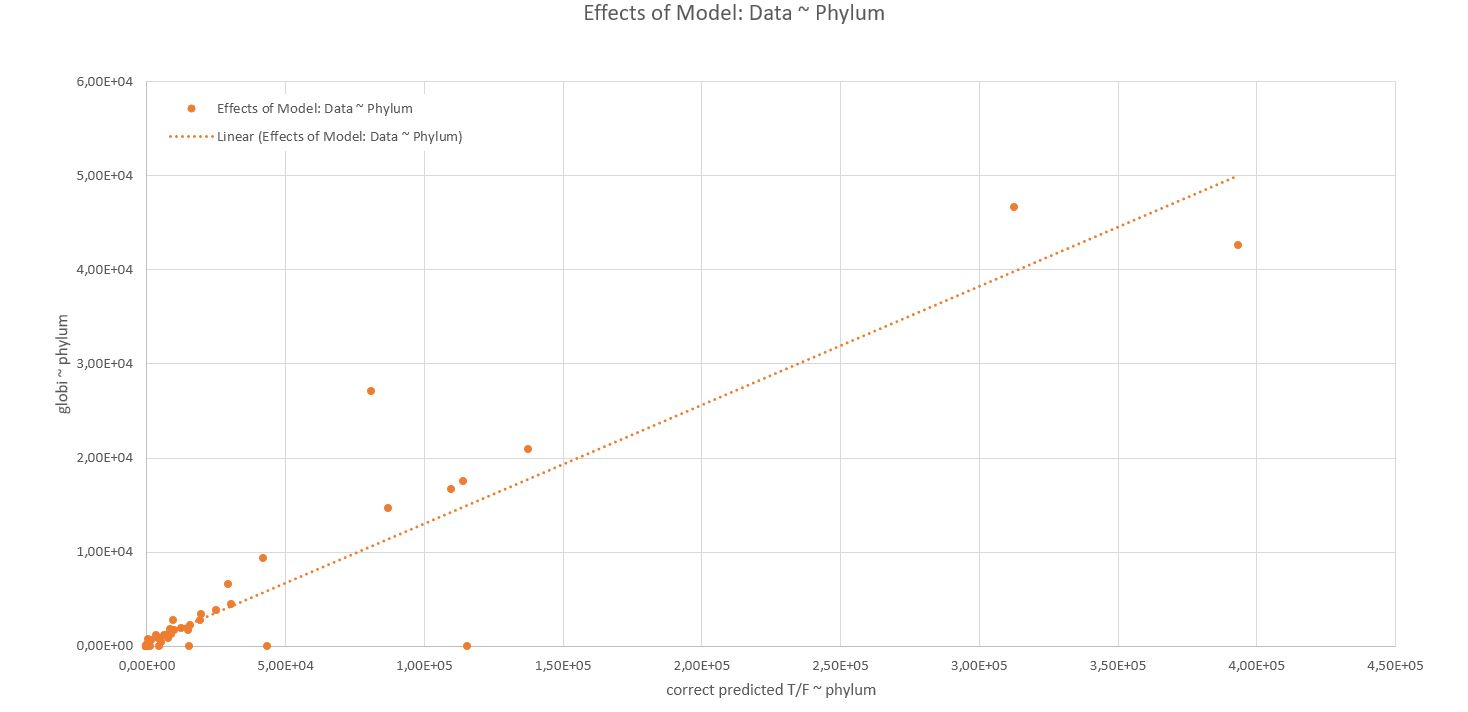
\includegraphics[trim = 0mm 0mm 0mm 15mm, clip, width=\textwidth]{Figures/EffectsOfModel-Data-Phylum.JPG}
      \caption{Effects of Model: Data $\sim$ Phylum}
      \label{fig:...}
    \end{figure}
    \begin{figure}[h!]
      \centering
      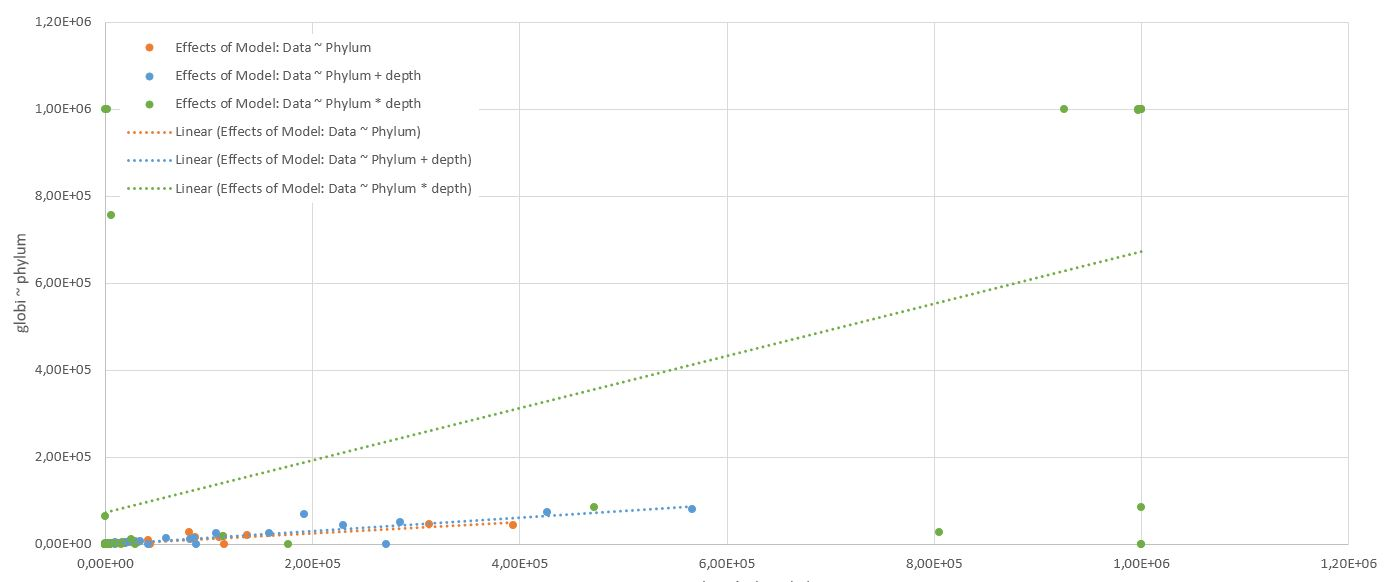
\includegraphics[trim = 0mm 0mm 0mm 0mm, clip, width=\textwidth]{Figures/EffectsOf3Models-Data-Phylum.JPG}
      \caption{Effects of 3 Models: Data $\sim$ Phylum (+/* depth)}
      \label{fig:...}
    \end{figure}
    \begin{figure}[h!]
      \centering
      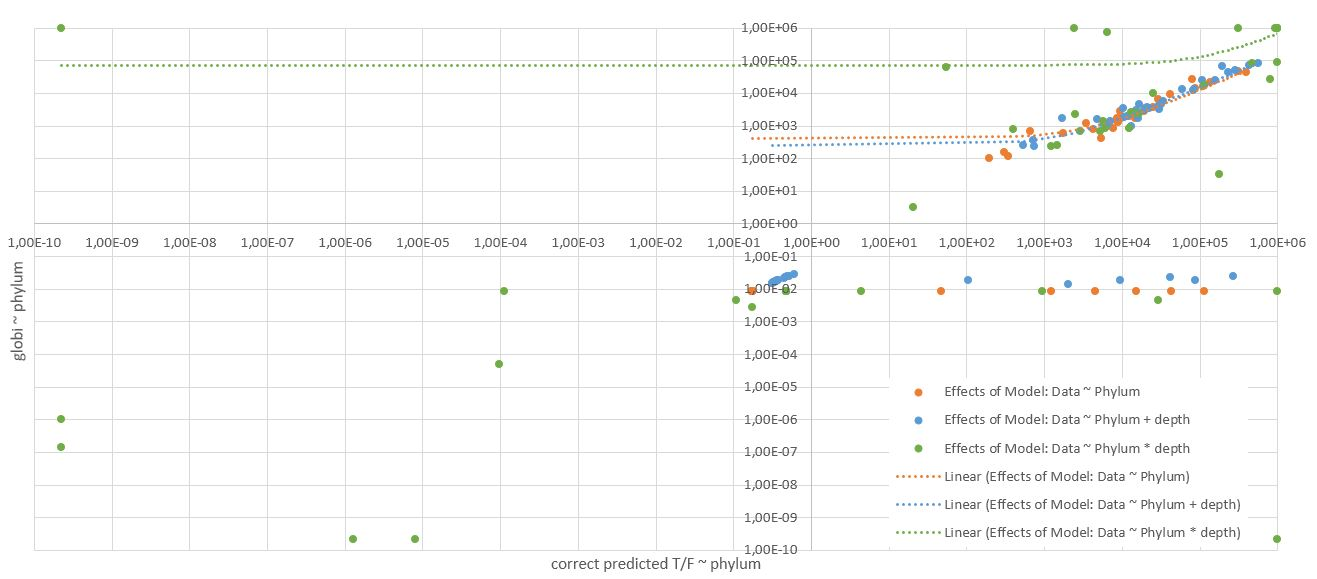
\includegraphics[trim = 0mm 0mm 0mm 0mm, clip, width=\textwidth]{Figures/EffectsOf3Models-Data-Phylum_loglog.JPG}
      \caption{Effects of 3 Models: Data $\sim$ Phylum (+/* depth) \\ both axis in log scale}
      \label{fig:...}
    \end{figure}

%---------------------------------------------------------------------------------------------------
%---------------------------------------------------------------------------------------------------
%---------------------------------------------------------------------------------------------------
%---------------------------------------------------------------------------------------------------
\chapter{Discussion}

  Fehlerqoute der Daten an sich? \\
  Wie gut ist unsere Datenlage? 3 mio knoten, 1.8 named species (leaf nodes), 200.000 leaf nodes mit 
  Information. \\
  Welche Teile des Baumes sind gut, an welchen muss noch viel geforscht werden. \\
  Wieviele Origins haben wir gefunden, was bedeutet diese Zahl? \\
  Es gibt noch ungenutze information in GloBI. \\
  Wir können GloBI verbessern ... Wir haben GloBI auf die gefundenen Abweichungen aufmerksam gemacht... 
    Fehler werden durch die prediction eventuell verstärkt...\\

  %---------------------------------------------------------------------------------------------------
  %---------------------------------------------------------------------------------------------------
  %---------------------------------------------------------------------------------------------------
  \section{Simulation}
    For fixed calculations we assume a distribution of 60\% free-living to 40\% parasites, 95\% 
      missing data and a multifuration rate of 95\%.
    How well does our simulation approach the real data situation? \\
    There are some points to discuss:
    \begin{itemize}
      \item How close is the randomized binary tree to a true phylogeny?
      \item The distribution of parasites to free-ranging species is a pure assumption. From different 
        sources about 40\% parasites are estimated, are these also beta-distributed?
      \item How well do the transition probabilities match parasitism? Depending on the type of 
        parasitism, this will certainly look different. In addition, it can be assumed that the 
        probability for losses is lower than for origins.
      \item The equal distribution of the multifurcation is a blank assumption. It is very likely to 
        be higher towards the root node because there is less information back in time. On the other 
        hand, there are many studies that have studied various species without considering phylogeny. 
        Which also creates a high number of children of a node directly at the leaf nodes.
    \end{itemize}
    In order to be able to observe these problems, we have programmed our simulation according to the 
      parameters. This allowed us to estimate the influence of some of these parameters.

  
%---------------------------------------------------------------------------------------------------
%---------------------------------------------------------------------------------------------------
%---------------------------------------------------------------------------------------------------
\bibliography{bibliographie}

%---------------------------------------------------------------------------------------------------
%---------------------------------------------------------------------------------------------------
%---------------------------------------------------------------------------------------------------
\chapter{Appendices}
  %---------------------------------------------------------------------------------------------------
  %---------------------------------------------------------------------------------------------------
  \section{Methods overview}
    % \begin{figure}[h!]
    %   \centering
    %   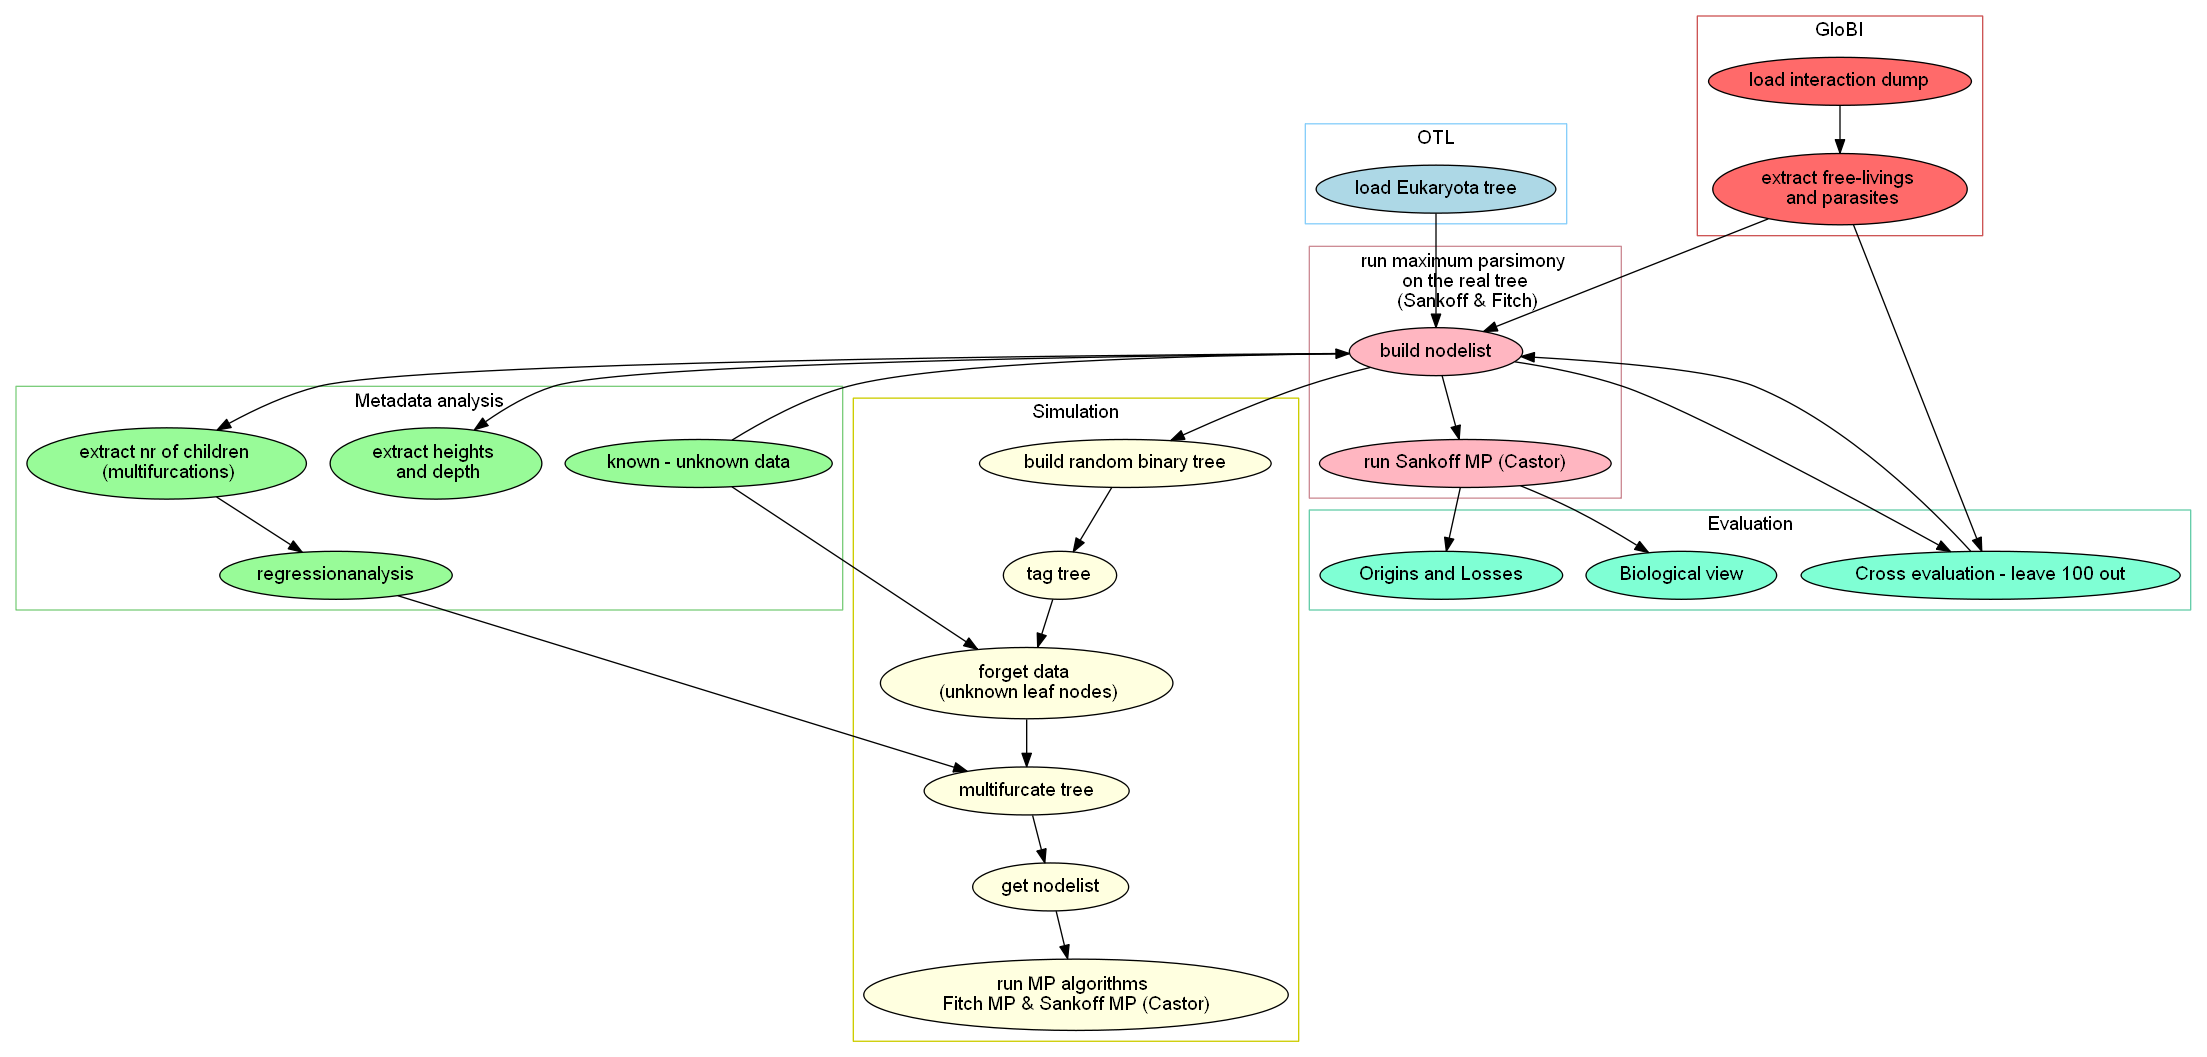
\includegraphics[angle=90, width=0.4\textwidth]{Figures/Workflow.png}
    %   \caption{Big overview of the whole Workflow}
    %   \label{fig:BigWorkflow}
    % \end{figure}
    \begin{figure}[h!]
      \centering
      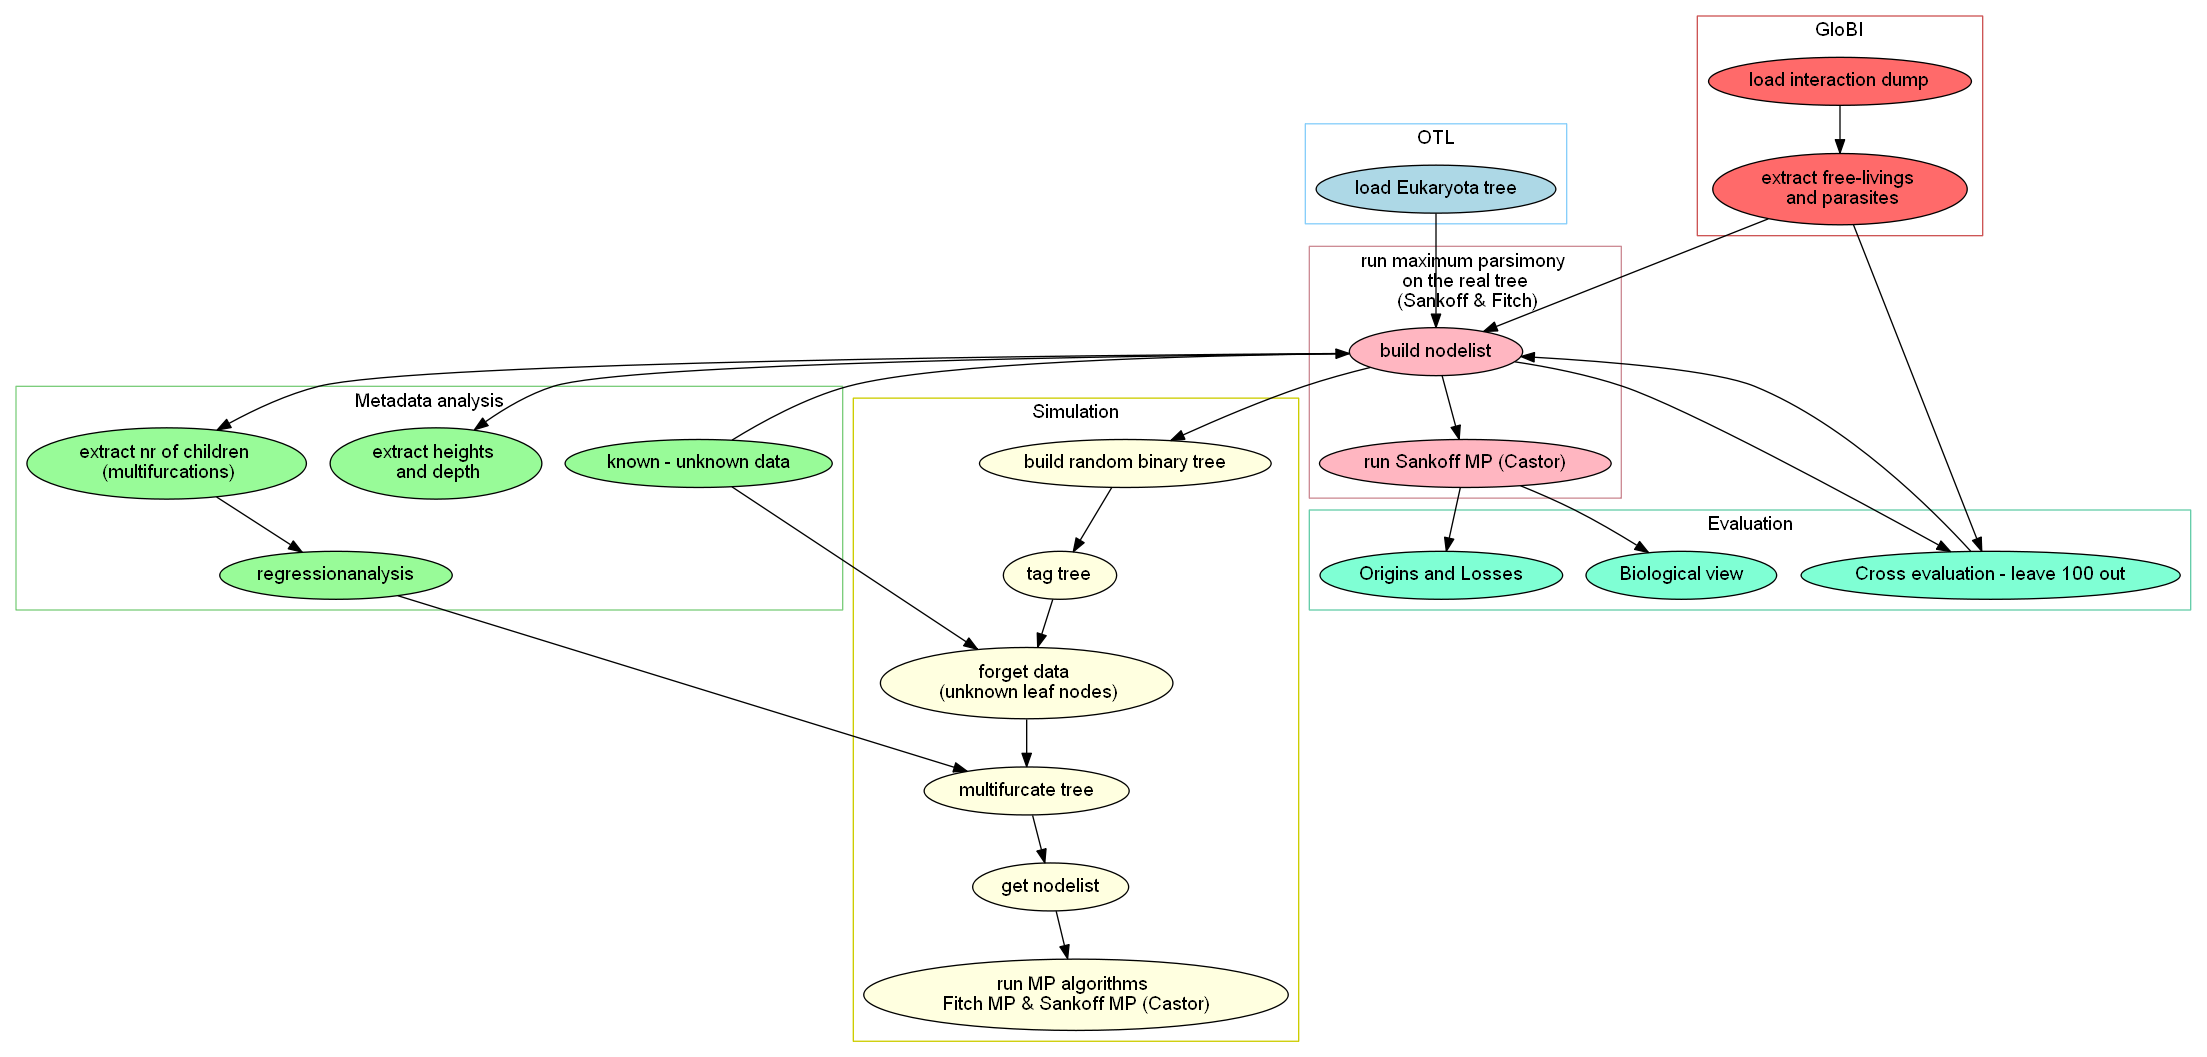
\includegraphics[width=\textwidth]{Figures/Workflow.png}
      \caption{Big overview of the whole Workflow}
      \label{fig:BigWorkflow}
    \end{figure}

  %---------------------------------------------------------------------------------------------------
  %---------------------------------------------------------------------------------------------------
  \section{OTL analysis}\label{sec:otl analysis}

    %---------------------------------------------------------------------------------------------------
    \subsection{List of all phyla}\label{subsec:listPhyla}

    Phyla (53): \\
    Acanthocephala, Amoebozoa, Apicomplexa, Arthropoda, Ascomycota, Bacillariophyta, Basidiomycota, 
      Brachiopoda, Bryozoa, Chaetognatha, Chlorophyta, Chordata, Chromerida, Chytridiomycota, 
      Ciliophora, Cnidaria, Colponemidia, Ctenophora, Cycliophora, Echinodermata, Entoprocta, 
      Entorrhizomycota, Euglenida, Foraminifera, Gastrotricha, Glomeromycota, Gnathostomulida, 
      Haplosporida, Haptophyta, Hemichordata, Kinorhyncha, Loricifera, Microsporidia, Mollusca, 
      Myzostomida, Nematoda, Nematomorpha, Nemertea, Onychophora, Orthonectida, Phaeophyceae, 
      Picozoa, Placozoa, Platyhelminthes, Porifera, Priapulida, Rhodophyta, Rhombozoa, Rotifera, 
      Streptophyta, Tardigrada, Xanthophyceae \\
    Wobei von Streptophyta -> Anthocerotophyta, Marchantiophyta, Bryophyta, Tracheophyta als
      Phylum im Phylum gefunden und nicht einbezogen wurden und Magnoliophyta als Phylum in 
      Tracheophyta ebenfalls nicht. \\

    %---------------------------------------------------------------------------------------------------
    \subsubsection{Distribution of Taxa}
    - In the tree we can distinguish 28 different Taxa with the OTL taxonomic tree. \\
    - The most of them are hardly represented. The major taxonomic groups are: ... \\
    - Here \colorbox{red}{you} can see some characteristics of the Multifurcation of the tree. \\
    \begin{figure}[h!]
      \centering
      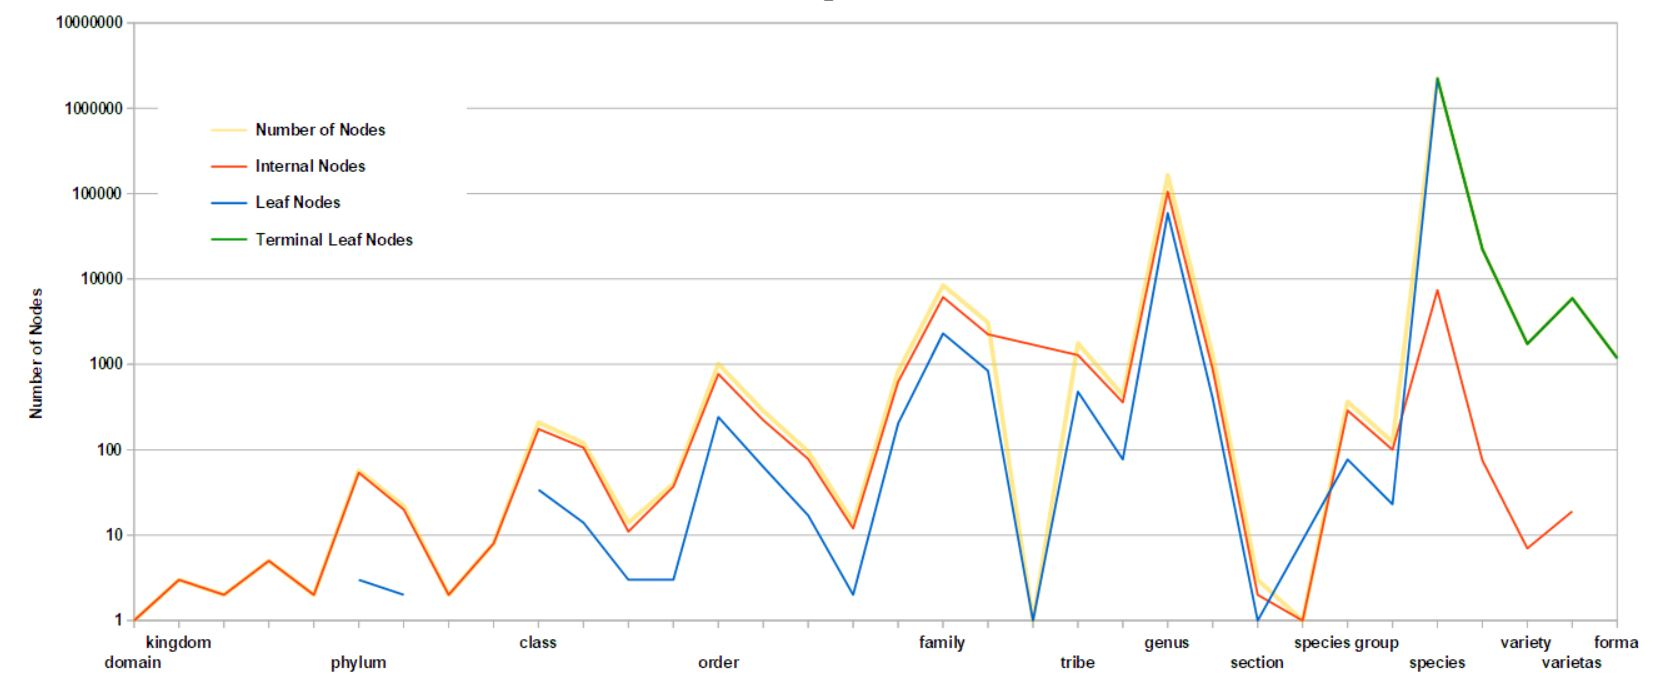
\includegraphics[width=0.9\textwidth]{Figures/TaxaTable2.JPG}
      \caption{Distribution of Nodes in Rank-Cathegories}
      \label{fig:taxaTable2}
    \end{figure}
    In a phylogeny, the taxonomic division of the tree is far too coarse, meaning that there should 
      be more subtaxa or 'unranked' nodes. But the closer we get to the root, the more the pure
      taxonomic tree is reflected. If the tree were binary, the taxa would have to double. But the 
      multipliers for some are much bigger and for others much smaller, which \colorbox{red}{you} can see in in figure 
      \ref{fig:taxaTable2}. \\
      ... (see Table \ref{table:...})
    
    \begin{table}[h!]
      \begin{center}
        % \begin{tabular}{ |>{\rowmac}l|>{\rowmac}r|<{\clearrow} }
        \begin{tabular}{ |l|r||r|r|r| }
          \hline
          Taxa & Number of Nodes & Internal Nodes & Leaf Nodes & Terminal Leaf Nodes \\
          \hline \hline
          \setrow{\bfseries}domain & 1 & 1 & &  \\ \hline
          \setrow{\bfseries}kingdom & 3 & 3 & &  \\
          subkingdom & 2 & 2 & & \\
          infrakingdom & 5 & 5 & & \\
          superphylum & 2 & 2 & & \\ \hline
          \setrow{\bfseries}phylum & 57 & 54 & 3 & \\
          subphylum & 22 & 20 & 2 & \\
          infraphylum & 2 & 2 & & \\
          superclass & 8 & 8 & & \\ \hline
          \setrow{\bfseries}class & 209 & 175 & 34 & \\
          subclass & 120 & 106 & 14 & \\
          infraclass & 14 & 11 & 3 & \\
          superorder & 40 & 37 & 3 & \\ \hline
          \setrow{\bfseries}order & 1014 & 772 & 242 & \\
          suborder & 285 & 222 & 63 & \\
          infraorder & 95 & 78 & 17 & \\
          parvorder & 14 & 12 & 2 & \\
          superfamily & 829 & 626 & 203 & \\ \hline
          \setrow{\bfseries}family & 8449 & 6143 & 2306 & \\
          subfamily & 3090 & 2250 & 840 & \\
          supertribe & 1 & 0 & 1 & \\
          tribe & 1764 & 1285 & 479 & \\
          subtribe & 435 & 359 & 77 & \\ \hline
          \setrow{\bfseries}genus & 164656 & 105452 & 59204 & \\
          subgenus & 1266 & 869 & 397 & \\
          section & 3 & 2 & 1 & \\
          subsection & 1 & 1 & 0 & \\
          species group & 365 & 288 & 77 & \\
          species subgroup & 123 & 100 & 23 & \\ \hline
          \setrow{\bfseries}species & 2247251 & 7423 & 2239828 & 2228993 \\
          subspecies & 22437 & 75 & 22362 & 22239 \\
          variety & 1755 & 7 & 1748 & 1726 \\
          varietas & 5970 & 19 & 5951 & 5909 \\
          forma & 1181 & & 1181 & 1181 \\
          \hline \hline
          no rank & 954 & 719 & 235 & 7 \\
          no rank - terminal & 37452 & & 37452 & 37452 \\
          (no entry) & 40099 & 40099 & & \\
          \hline  
        \end{tabular}
        \caption{\todo{...}}
        \label{table:...} 
      \end{center}  
    \end{table}
    extended leaf nodes (real leaf nodes)

  %---------------------------------------------------------------------------------------------------
  \subsubsection{Distribution of data in the taxa}
    Mithilfe des taxonomischen Baums von OTL haben wir die Knoten ihren Kingdoms, Phyla und Classes 
      zugeteilt (see Table \ref{table:...}). \\

    \begin{table}[h]
      \begin{center}
        \begin{tabular}{ |l|r|l|r|r| }
          \hline
          Kingdom (3) & Number of Nodes & Phylum (25) & Number of Nodes & max max height \\
          \hline \hline
          Metazoa & 1 465 207 & Arthropoda & 1 170 539 & 54 \\
          & & Chordata & 106 650 & 74 \\
          & & Mollusca & 80 022 & 22 \\
          & & Platyhelminthes & 27 141 & 9 \\
          & & Nematoda & 24 564 & 23 \\
          & & Cnidaria & 14 878 & 36 \\
          & & Porifera & 11 737 & 26 \\
          & & Echinodermata & 10 654 & 14 \\
          & & Bryozoa & 8 631 & 11 \\
          & & Rotifera & 3 093 & 7 \\
          & & Nemertea & 1 793 & 7 \\
          & & Tardigrada & 1 654 & 7 \\
          & & Acanthocephala & 1 596 & 6 \\
          & & Brachiopoda & 1 055 & 9 \\
          & & Nematomorpha & 633 & 7 \\
          & & Chaetognatha & 360 & 7 \\
          & & Hemichordata & 196 & 5 \\ 
          & & Cycliophora & 11 & 5 \\ 
          % 1465207-(1170539+106650+80022+27141+24564+14878+11737+10654+8631+3093+1793+1654+1596+1055+633+360+196+11) = 0          \hline
          Fungi & 254 871 & Ascomycota & 157 045 & 19 \\ 
          & & Basidiomycota & 92 931 & 18 \\
          & & Microsporidia & 1 949 & 6 \\ 
          & & Glomeromycota & 1 490 & 6 \\
          & & Chytridiomycota & 1 456 & 6 \\
          % 254871-157045-92931-1949-1490-1456 = 0
          \hline
          Chloroplastida & 121 239 & Streptophyta & 120 731 & 49 \\
          & & Chlorophyta & 508 & 6 \\
          % 121239-120731-508 = 0
          \hline  
        \end{tabular}
        \caption{\todo{...}}
        \label{table:...} 
      \end{center}  
    \end{table}

  %---------------------------------------------------------------------------------------------------
  %---------------------------------------------------------------------------------------------------
  \section{Missing leaf state modelling - Resiudal tables}\label{sec:Residuals unknown information}

    \begin{table}[h!]
      \begin{center}
        \begin{tabular}{ |l|r|r|r| }
          \hline
          Model / Taxa & Kingdom & Phylum & Class \\
          \hline \hline
          multifurc $\sim$ taxa & 545740 & \cellcolor{green!10}499227 & \cellcolor{green!30}482265 \\
          \hline
          multifurc $\sim$ taxa + depth & 544789 & \cellcolor{green!10}493017 & \cellcolor{green!50}478998 \\
          \hline
          multifurc $\sim$ taxa * depth & 544062 & \cellcolor{green!30}488366 & \cellcolor{green!50}476382 \\
          \hline
        \end{tabular}
      \end{center}
      \caption{Residuals of unknown information}
    \end{table}


\end{document}